%%%%%%%%%%%%%%%%%%%%%%%%%%%%%%%%%%%%%%%%%%%%%%%%%%%%%%%%%%%%
%%% LIVECOMS ARTICLE TEMPLATE FOR BEST PRACTICES GUIDE
%%% ADAPTED FROM ELIFE ARTICLE TEMPLATE (8/10/2017)
%%%%%%%%%%%%%%%%%%%%%%%%%%%%%%%%%%%%%%%%%%%%%%%%%%%%%%%%%%%%
%%% PREAMBLE
\documentclass[9pt,bestpractices]{livecoms}
% Use the 'onehalfspacing' option for 1.5 line spacing
% Use the 'doublespacing' option for 2.0 line spacing
% Use the 'lineno' option for adding line numbers.
% The 'bestpractices' option for indicates that this is a best practices guide.
% Omit the bestpractices option to remove the marking as a LiveCoMS paper.
% Please note that these options may affect formatting.

\usepackage{lipsum} % Required to insert dummy text
\usepackage[version=4]{mhchem}
\usepackage{siunitx}
\DeclareSIUnit\Molar{M}
\usepackage[italic]{mathastext}
\graphicspath{{figures/}}

%%%%%%%%%%%%%%%%%%%%%%%%%%%%%%%%%%%%%%%%%%%%%%%%%%%%%%%%%%%%
%%% IMPORTANT USER CONFIGURATION
%%%%%%%%%%%%%%%%%%%%%%%%%%%%%%%%%%%%%%%%%%%%%%%%%%%%%%%%%%%%
\usepackage[colorinlistoftodos]{todonotes}
\newcommand{\versionnumber}{0.1}  % you should update the minor version number in preprints and major version number of submissions.
\newcommand{\githubrepository}{\url{https://github.com/michellab/alchemical-best-practices}}  %this should be the main github repository for this article
\newcommand{\expect}[1]{\left\langle{#1}\right\rangle}
%%%%%%%%%%%%%%%%%%%%%%%%%%%%%%%%%%%%%%%%%%%%%%%%%%%%%%%%%%%%
%%% ARTICLE SETUP
%%%%%%%%%%%%%%%%%%%%%%%%%%%%%%%%%%%%%%%%%%%%%%%%%%%%%%%%%%%%
\title{Best Practices for Alchemical Free Energy Calculations: v\versionnumber}
\author[7]{Bryce K. Allen}
\author[1*]{John D. Chodera}
\author[2,12]{Maximilian Kuhn}
\author[2*]{Antonia S. J. S. Mey}
\author[2*]{Julien Michel}
\author[3*]{David L. Mobley}
\author[1]{Levi N. Naden}
\author[4*]{Samarjeet Prasad}
\author[5*]{Julia E. Rice}
\author[1,9]{Andrea Rizzi}
\author[2*]{Jenke Scheen}
\author[6*]{Michael Shirts}
\author[11]{Gary Tresadern}
\author[10*]{Huafeng Xu}



\affil[1]{Computational and Systems Biology Program, Sloan Kettering Institute, Memorial Sloan Kettering Cancer Center, New York NY, USA}
\affil[2]{EaStCHEM School of Chemistry, David Brewster Road, Joseph Black Building, The King's Buildings, Edinburgh, EH9 3FJ, UK}
\affil[3]{Departments of Pharmaceutical Sciences and Chemistry, University of California, Irvine, USA}
\affil[4]{National Institutes of Health, Bethesda, MD, USA}
\affil[5]{IBM Alamden Research Center, Almaden, CA, USA}
\affil[6]{University of Colorado Boulder, Boulder, CO, USA}
\affil[7]{Silicon Therapeutics, Boston, MA, USA}
\affil[8]{Tri-Institutional Training Program in Computational Biology and Medicine, New York, NY, USA}
\affil[11]{Computational Chemistry, Janssen Research & Development, Turnhoutseweg 30, Beerse B-2340,Belgium}


\corr{john.chodera@choderalab.org}{JDC}
\corr{dmobley@mobleylab.org}{DLM}
\corr{antonia.mey@ed.ac.uk}{ASJSM}
\corr{mail@julienmichel.net}{JM}
\corr{michael.shirts@colorado.edu}{MRS}

\contrib[\authfn{1}]{These authors contributed equally to this work}
\contrib[\authfn{2}]{These authors also contributed equally to this work}


\blurb{This LiveCoMS document is maintained online on GitHub at \githubrepository; to provide feedback, suggestions, or help improve it, please visit the GitHub repository and participate via the issue tracker.}

%%%%%%%%%%%%%%%%%%%%%%%%%%%%%%%%%%%%%%%%%%%%%%%%%%%%%%%%%%%%
%%% PUBLICATION INFORMATION
%%% Fill out these parameters when available
%%% These are used when the "pubversion" option is invoked
%%%%%%%%%%%%%%%%%%%%%%%%%%%%%%%%%%%%%%%%%%%%%%%%%%%%%%%%%%%%
\pubDOI{10.XXXX/YYYYYYY}
\pubvolume{<volume>}
\pubyear{<year>}
\articlenum{<number>}
\datereceived{Month, Day, Year}
\dateaccepted{Month, Day, Year}

%%%%%%%%%%%%%%%%%%%%%%%%%%%%%%%%%%%%%%%%%%%%%%%%%%%%%%%%%%%%
%%% ARTICLE START
%%%%%%%%%%%%%%%%%%%%%%%%%%%%%%%%%%%%%%%%%%%%%%%%%%%%%%%%%%%%

\begin{document}

\begin{frontmatter}
\maketitle

\begin{abstract}
Alchemical free energy calculations can be a useful tool for predicting free energy differences associated with the transfer of small molecules from one environment to another.
The hallmark of these methods is the use of modified potential energy functions to represent \emph{alchemical} intermediate states that cannot exist in chemistry; by analyzing simulation data collected from a series of bridging alchemical thermodynamic states, transfer free energies (or differences in transfer free energies) can be computed with orders of magnitude less simulation time than observing the process spontaneously. 
While these methods are highly flexible, care must be taken in avoiding common pitfalls to ensure that computed free energy differences can be robust and reproducible for the chosen forcefield, and that appropriate corrections are included to permit direct comparison with experimental data.
In this paper, we review current best practices for several popular application domains of alchemical free energy calculations, including relative and absolute small molecule binding free energy calculations to biomolecular targets.
\todo[inline, color=green!20]{JDC: Should we migrate this document to \url{https://github.com/alchemistry}? ASJSM: Let's migrate with the submitted version, but leave it here for now?}
\end{abstract}

\end{frontmatter}
https://www.overleaf.com/5136551543vgjqbkzpmqkp


\todototoc
\listoftodos

%%%%%%%%%%%%%%%%%%%%
%  Introduction    %
%%%%%%%%%%%%%%%%%%%%
\section{What are alchemical free energy methods?}
\label{sec:intro}
Alchemical free energy (FE) calculations allow the calculation of energy differences associated with changes from one state to another, such as ligand binding to protein from solvent~\cite{zwanzig1954hightemperature}. The calculations use non-physical intermediate states where atoms are changed from one to another or can be removed or inserted by decoupling or coupling with their environment, Figure 1. These so-called alchemical states permit converged calculations for large changes, such as the entire removal of a ligand from a binding site, known as an absolute FE calculation, or modifying a substituent between two analogous ligands in a binding site, a relative FE calculation. Two common approaches are free energy perturbation (FEP) and thermodynamic integration (TI) for which the theory dates back decades but with the first computational applications emerging in the 1980's and 90's~\cite{kirkwood1935statistical, jorgensen1985monte, kollman1993free, wong1986dynamics, merz1989free}. Important studies continued during the 2000's often leading to improved implementation of the methods in common simulation software~\cite{vanderspoel2005gromacs, mermelstein2018fast, wang2015accurate, biosimspace}. This foundation work, combined with the methodological, technological and hardware improvements of the last 5-10 years have led to an explosion of interest.  The domain of applicability for these calculations now involves such varied applications as the computation of protein-ligand binding free energies (both relative~\cite{relative-binding-free-energies} and absolute~\cite{absolute-binding-free-energies}), ligand selectivities~\cite{selectivity}, partition and distribution coefficients between different liquid phases (such as octanol-water partition coefficients~\cite{octanol-water-partition}), affinity changes due to mutations in therapeutic targets~\cite{hauser2018predicting,aldeghi2018accurate}, and changes in protein thermostability~\cite{seeliger2010protein,gapsys2016insights,gapsys2016accurate,aldeghi2019accurate}. As the field of molecular simulation moves towards millisecond timescales accurate FE calculations on even more challenging problems will be in scope. In the meantime, today's user may find it hard to get started with these complex calculations whilst also keeping up with the fast pace of change. This best practice guide aims to serve as a go-to reference for current recommendations and tips for users of all experience.  

\begin{figure}
    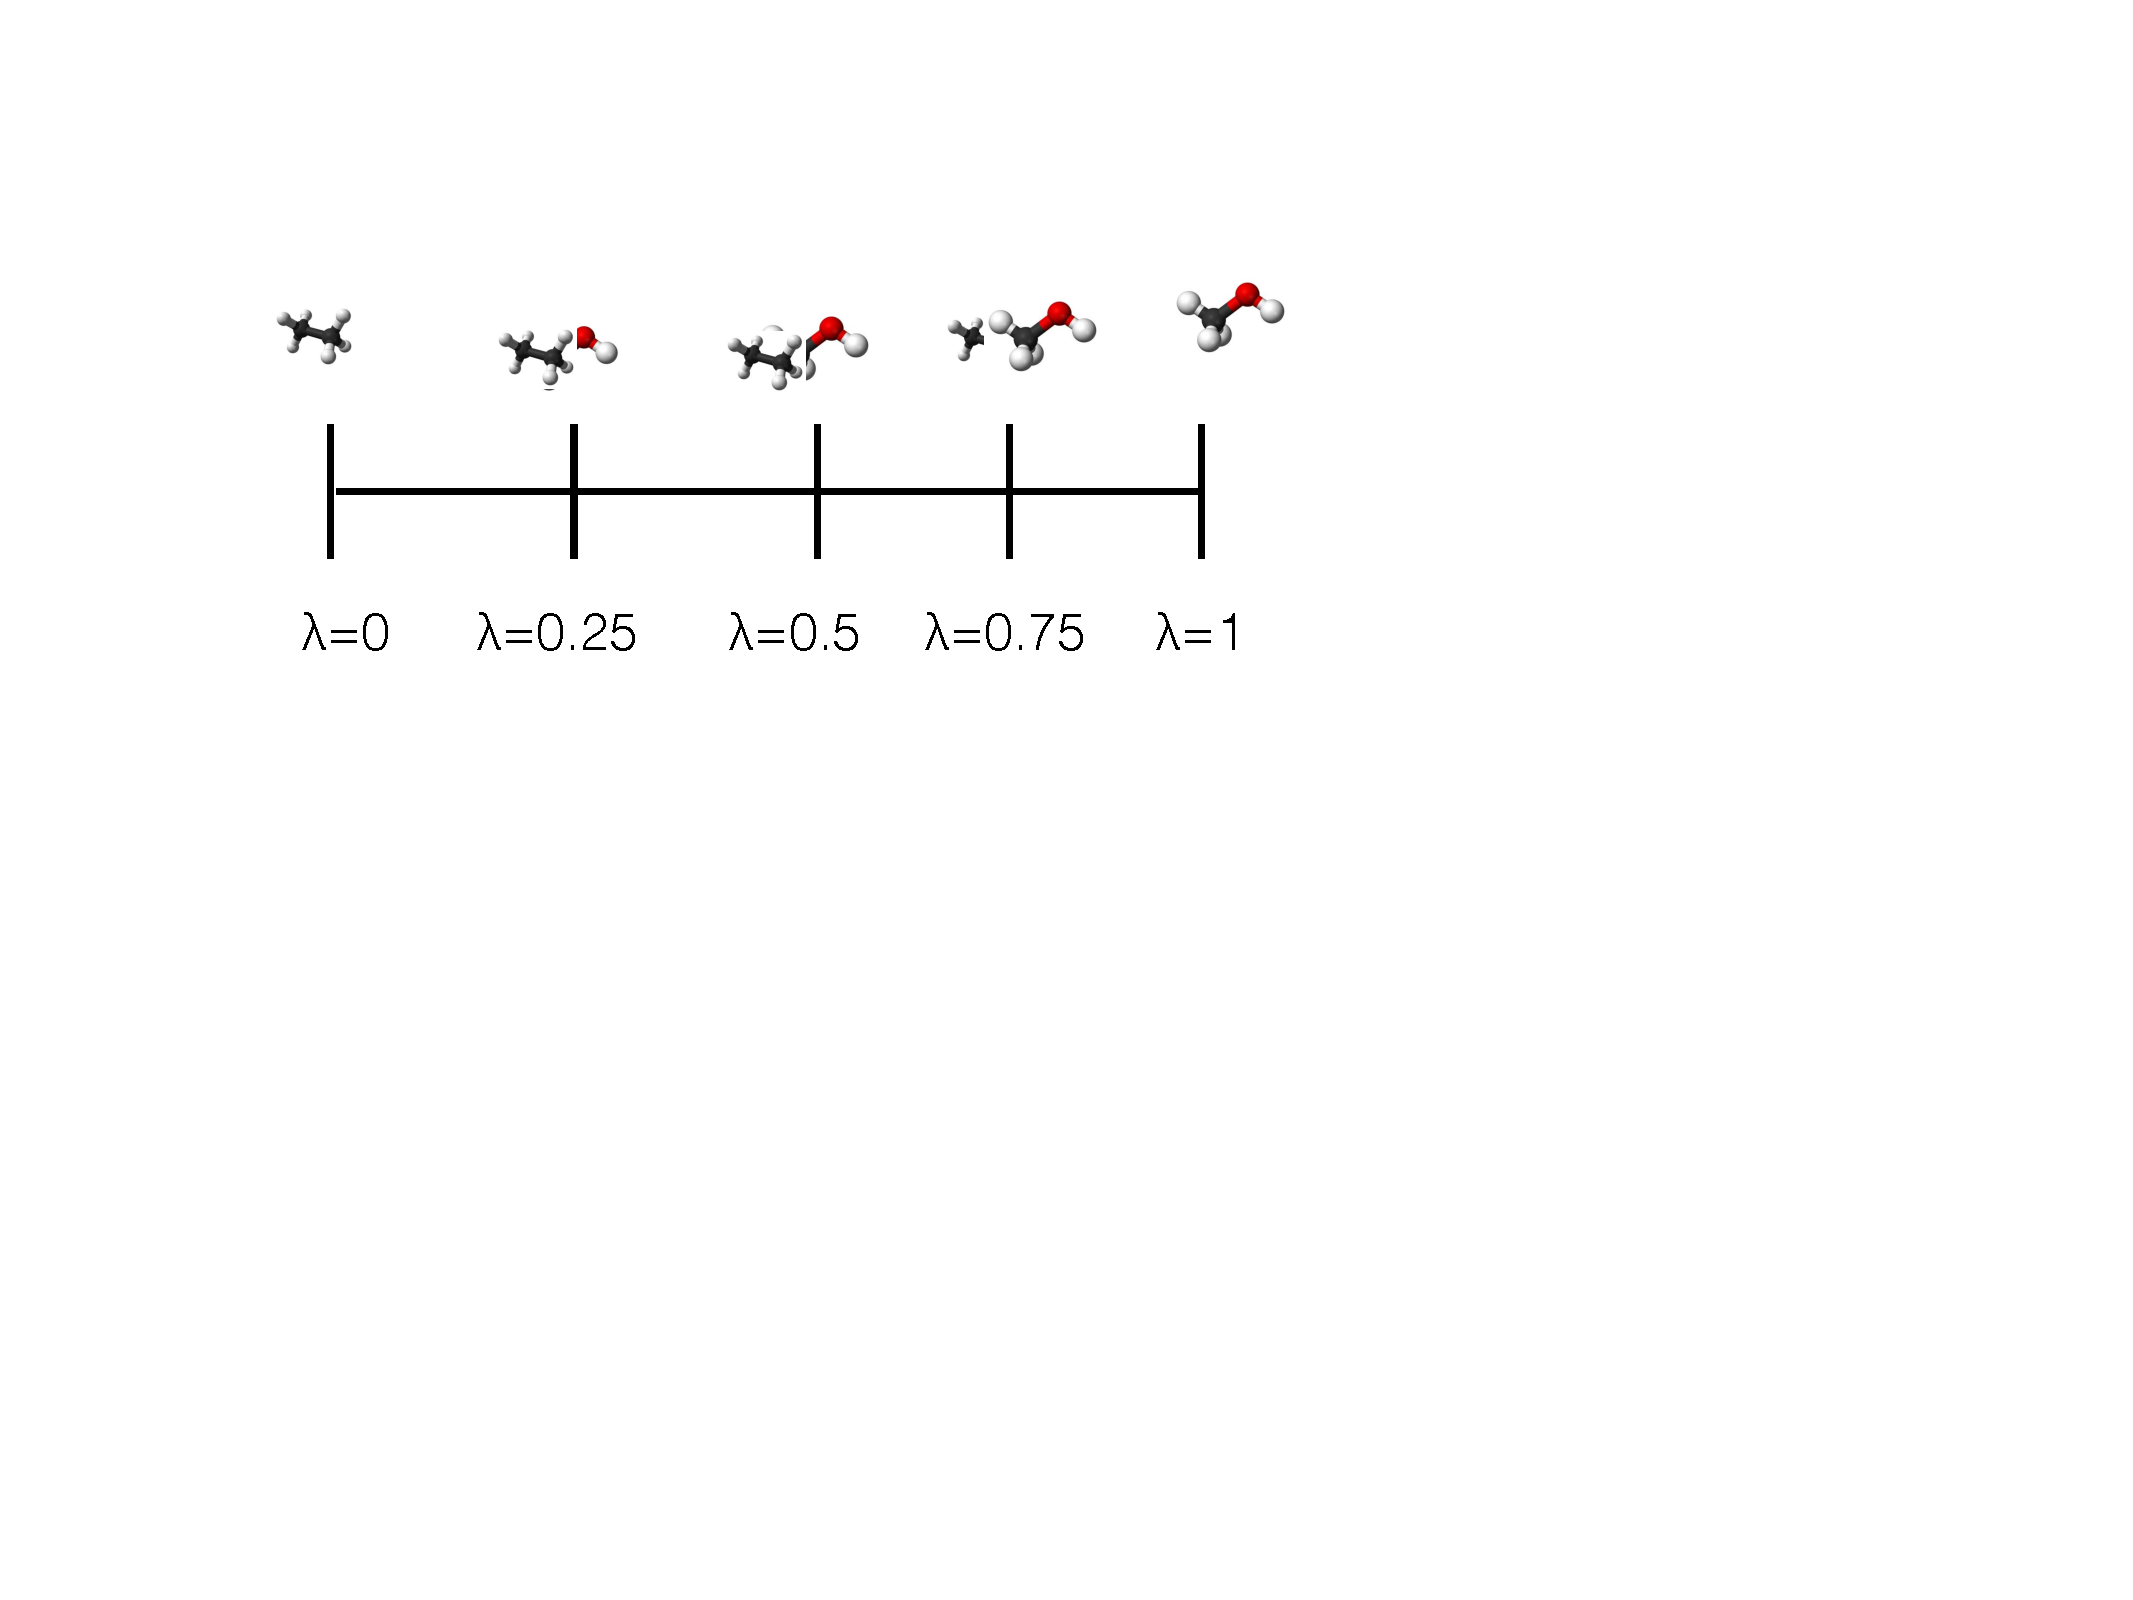
\includegraphics[width=0.95\linewidth]{figures/fig1/Fig1_dummy.pdf}
    \caption{{\bf What is alchemistry?}
    \todo[inline, color=green!20]{JDC: What is the concept for what this figure is supposed to communicate?}
    }
    \label{fig:fig1}
\end{figure}

\todo[inline, color={green!20}]{ASJSM: This section should be expanded a little, but in a very general way, any volunteers?}

%%%%%%%%%%%%%%%%%%%%
% Prerequesites    %
%%%%%%%%%%%%%%%%%%%%
\section{Prerequisites and Scope}
\label{sec:pre}
%Here you would identify prerequisites/background knowledge that are assumed by your work and your checklist which you view as critical, ideally giving links to good sources on these topics.
%Checklists are normally focused on errors made by users with training and experience in molecular simulations, so you can assume a basic familiarity with the fundamentals of molecular simulations.

\todo[inline, color={green!20}]{JDC: This section could benefit from further refinement to ensure it is fully internally consistent.}

This best practices guide aims to answer the following questions:
\begin{itemize}
    \item Is my problem suitable for an alchemical free energy calculation? 
    \item How do I chose the right free energy protocol and run it? How do I analyze my simulations accurately? 
    \item What software tools are available to simulate alchemical free energy protocols? 
\end{itemize}
This guide is meant to serve as a comprehensive starting point for new practitioners, as well as a reference guide with a convenient checklist (Section~\ref{sec:checklist}) to help with standard alchemical simulation and analysis practices. 
We will also give a brief overview of available software packages and their corresponding capabilities.
The checklist we provide can serve as a good guide for a methods section both to the author of a free energy paper as well as a reviewer. 
\todo[inline, color={green!20}]{JDC: Do we only describe software that allows these best practices to be implemented in totality, or do we highlight when certain practices cannot be implemented in software we describe? Asjsm: where this is known we should do this.}

We assume the reader possesses a basic familiarity with the principles of molecular mechanics, molecular dynamics simulations, statistical mechanics, and the biophysics of protein-ligand association.
For readers unfamiliar with these concepts that have never set up and run an equilibrium molecular dynamics simulation, we would recommend the following texts for getting started with these topics first. 
\begin{itemize}
    \item Statistical mechanics and thermodynamics background~\cite{hill1956statistical, alavi2011statistical}
    \item Understanding theory of how molecular simulations work~\cite{frenkel2002understanding}
    \item Docking reviews~\cite{yuriev2013latest, meng2011molecular} and software overview~\cite{pagadala2017software} and generating valid molecular structures ~\cite{loeffler2015fesetup}
    \item Getting started with setting up and running equilibrium molecular dynamics simulations: Gromacs tutorial~\cite{lemkul2018From}, Amber tutorial~\cite{amber}, HTMD: high-throughput Molecular Dynamics for Molecular Discovery~\cite{doerr2016htmd}*, or with VMD and NAMD~\cite{ribeiro2016easy}*
\end{itemize}
References marked with an asterisk (*) indicate nonessential reading or tutorials that provide further depth and understanding.

As some of the theoretical background can seem daunting, we provide an essentials guide to the theory behind alchemical fee energy calculations in Section~\ref{sec:theory}. 
We will cover topics that are essential to the  preparation, execution, and analysis of alchemical free energy calculations. 
Particular focus will be given to aspects of the molecular simulations which are unique to alchemical calculations---these include the calculation of transfer free energies (hydration free energies, partition coefficients, etc.), and binding free energies (absolute and relative).
While we try to address as many methods and practices as possible, the field of free energy calculations is broad, and there are many advanced topics that are left to future best practices documents focusing on specific issues. 

Below, we provide a non-exhaustive list of topics we have not addressed with some references to provide starting points on these more advanced topics:
\begin{itemize}
\item Covalent inhibition.
\item Complex association stoichiometry (beyond simple 1:1 association)~\cite{awesome reference}. 
\item Endpoint free energy methods such as MM-PBSA~\cite{genheden2015mm} and LIE~\cite{gutierrez-de-terran2012linear}
\item Free energy methods that extract the ligand using geometric order parameters and potential of mean force methods~\cite{heinzelmann2017attachpullrelease}
\item Forcefield dependence for protein, ligand, ions, co-solvents, and co-factors. Different studies have looked at the influence of force fields and we assume you made an adequate choice for the system you would like to study.~\cite{loeffler2018reproducibility, vassetti2019assessment, lopes2015current} 
\end{itemize}

%%%%%%%%%%%%%%%%%%%%
% Theory basics    %
%%%%%%%%%%%%%%%%%%%%

\section{Theoretical background}
\label{sec:theory}
\todo[inline, color={green!20}]{Info box what is free energy}
\todo[inline, color={green!20}]{Info box what is a thermodynamic cycle}

$\left[
      \begin{tabular}{@{\quad}m{0.8\columnwidth}@{\quad}}
          \raggedright%
          \textbf{What is a thermodynamic cycle?} \par
            There's a package called \texttt{url} designed for typesetting web addresses.
            Write \mbox{\texttt{\string\usepackage\string{url\string}}} in your preamble; this will provide the
            command \mbox{\texttt{\string\url}}. This command takes an address for the argument and
            will print it out with typewriter font. Furthermore, it is able to handle
            special characters in addresses like underscores and percent signs. It even
            enables hyphenation in addresses, which is useful for websites with a very
            long name.%
      \end{tabular}
\right]$
\newline
%May need to look at this again: https://tex.stackexchange.com/questions/66820/how-to-create-highlight-boxes-in-latex
The defining characteristic of alchemical free energy calculations is the use of a series of alchemically-modified potential functions $U(x; \lambda)$ in which an alchemical parameter $\lambda$ modulates interactions in a manner that cannot occur in real chemical systems.
One or more simulations are used to collect data from a multitude of alchemical states to compute a free energy difference between a chemical state ($\lambda_0$) and another chemical or alchemical reference state ($\lambda_1$),
\begin{eqnarray}
\Delta f &\equiv& f(\lambda_1) - f(\lambda_0) = - \ln \frac{Z(\lambda_1)}{Z(\lambda_0)} , \label{equation:dimensionless-free-energy-difference}
\end{eqnarray}
where the dimensionless free energy $f(\lambda) \equiv \beta F(\lambda)$ is given in terms of partition functions $Z(\lambda)$,
\begin{eqnarray}
Z(\lambda) &=& \int dx \, e^{-u(x; \lambda)} . \label{equation:partition-function-definition}
\end{eqnarray}
Here, the inverse thermal energy $\beta \equiv (k_B T)^{-1}$ where $k_B$ is the Boltzmann constant and $T$ is the absolute temperature, and the \emph{reduced potential} $u(x; \lambda)$~\cite{shirts2008statistically} is generally given by a trace over thermodynamic parameters with their conjugate dynamical variables,
\begin{eqnarray}
u(x;\lambda) &\equiv& \beta \left[ U(x;\lambda) + p \, V(x) + \sum_{i=1}^N \mu_i \, N_i(x) + \cdots \right] . \label{equation:reduced-potential}
\end{eqnarray}
Here, the collection of thermodynamic and alchemical parameters $\theta \equiv \{\beta, \lambda, p, \mu, \ldots\}$ defines a \emph{thermodynamic state}.
The physical transformation of interest---such as a protein-ligand association process, or transfer free energy among phases---may involve a thermodynamic cycle that requires several free energy differences $\Delta f$ to be computed in order to produce an estimate of the overall desired quantity.

\begin{figure}
    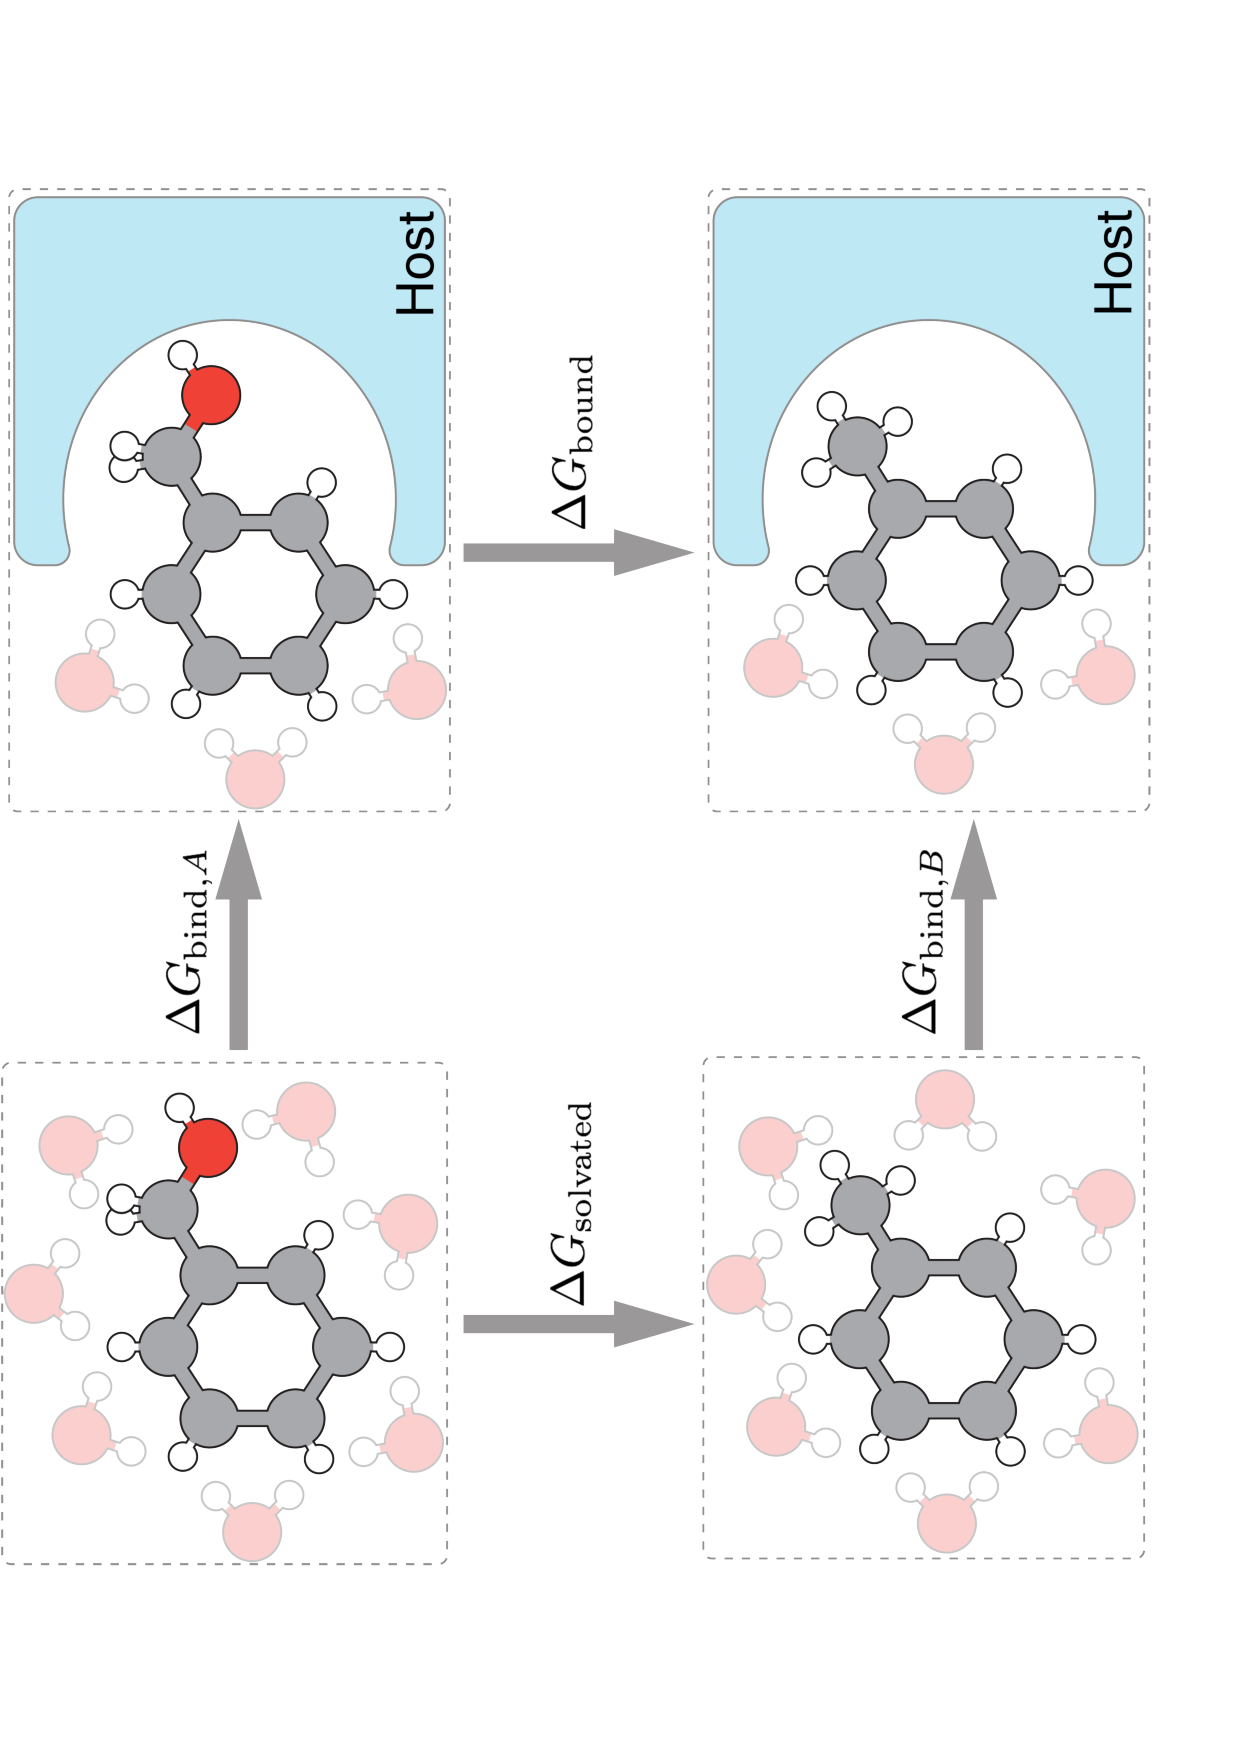
\includegraphics[width=0.95\columnwidth]{paper/figures/fig2/Fig2.pdf}
    \caption{{\bf Thermodynamic cycle for computing the relative free energy of binding ($\Delta \Delta G$) between two related small molecules to a supramolecular host.}
    The relative binding free energy difference between two small molecules, $\Delta \Delta G_{\mathrm{bind}, A \rightarrow B} \equiv \Delta G_{\mathrm{bind}, B} - \Delta G_{\mathrm{bind}, A}$---here benzyl alcohol (top) to toluene (bottom)---can be computed as a difference between two alchemical transformations, $\Delta G_\mathrm{bound} - \Delta G_\mathrm{solvated}$, where $\Delta G_\mathrm{bound}$ represents the free energy change of transforming $A \rightarrow B$ in complex and $\Delta G_\mathrm{solvated}$ the free energy change of transforming $A \rightarrow B$ in solvent.}
    \label{fig:fig1}
\end{figure}
\todo[inline, color=green!20]{This section needs to be expanded and give a good introduction to the theoretical background without going into too much detail.}


%%%%%%%%%%%%
% Step 0   %
%%%%%%%%%%%%
\section{What can be expected from alchemical simulations? -- Step 0}
\label{sec:step0}
\todo[inline, color={green!20}]{@everyone please review this section}
Step 0 is essentially about initially counting the cost of your
project: Can you even hope to tackle the problem you are thinking
about attempting given available resources and, if successful, will it
be worth it?
\subsection*{How accurate are current alchemical free energy calculations?}
Current alchemical free energy calculations seem to achieve, in favorable cases, RMS errors around 1-2 kcal/mol depending on force field, system, and a variety of other factors such as simulation time, sampling method, and whether the calculations employed are absolute or relative~\cite{lots-of-citations}. 
\todo[inline,color={green!20}]{JDC: We should probably provide a short list of key benchmark references here, broken down by force field, and keep this up to date. GT: would a table, at the end of the document be an easier way to do this, only requiring some brief comments in the text?}
However, the domain of applicability is a significant concern~\cite{Sherborne2016, Cournia2017}, especially for relative calculations, which typically require a bound structure of a closely
related ligand as a starting point. Additional factors such as slow protein or ligand rearrangements, uncertainties in ligand binding mode, or charged ligands can make these calculations far less reliable and more of a research effort.

It is worth noting that the accuracy of free energy calculations is highly variable across different protein targets, and likely across different ligand chemotypes as well. For instance, FEP+ with OPLS3 achieves an RMSE of 0.62 kcal/mol for a set of 21 compounds binding to JNK1 kinase, yet only an RMSE of 1.05 kcal/mol for a set of 34 compounds binding to P38$\alpha$ kinase (cite Harder et al. 2016). Furthermore, perturbations for the same chemotype in different pockets of the BACE enzyme gave varied errors (cite keranen et al jctc 2017, 13 1439)  
\todo[inline,color={green!20}]{JDC: It's important to be clear on what error is being reported: $\Delta G$ after shifting by a constant to minimize the RMSE, unshifted $\Delta G$, $\Delta \Delta G$ of computed edges, or $\Delta \Delta G$ of all edges. Note that computed edge $\Delta \Delta G$ RMSE significantly underestimates the error of all edge RMSE: \url{https://github.com/jchodera/jacs-dataset-analysis}}
We
thus recommend that retrospective study for a particular target and a particular chemical series be performed to establish the relevant accuracy of free energy calculations for each particular application case.

\subsection{Is the system of study suitable for alchemical free energy calculations?}
Before even planning free energy calculations to study binding to a
particular target, it is important to assess what is known about the
system and its timescales and its suitability for free energy
calculations, as well as the \emph{purpose} of the calculations and
the amount of available computer resources. In some cases, predicting
accurate binding free energies for a particular target might be a
\emph{more} challenging effort than simply measuring them! This is
often the case when dealing with database screening problems, where
compounds might be easily and quickly available commercially for
testing and free energy calculations could consume a much larger
amount of resources. Free energy calculations thus typically only
appeal when (slow or costly) synthesis would be required to do
experiments or experiments are otherwise cost-prohibitive.

Sometimes free energy calculations can provide answers that are not
readily available from experiments.  For example, type II kinase
inhibitors selectively bind to different kinases in the so-called
DFG-out conformations (cite Kuriyan).  The selectivity of such
inhibitors may be attributed either to their differential binding to
different kinases in the DFG-out conformations, or to different
stability of the DFG-out conformations of different kinases.  Let
$K_C$ be the equilibrium constant between DFG-in and DFG-out
conformations of one kinase, and $K_D^\ast$ be the dissociation
constant of a type II inhibitor against this kinase, the apparent
binding constant of this inhibitor against this kinase is then
\begin{equation}
  K_D = K_D^\ast \frac{1 + K_C}{K_C}
  \label{eqn:conformational-binding}
\end{equation}

Since binding experiments cannot resolve $K_D^\ast$ and $K_C$ individually,
such experiments cannot address the basis of selectivity of the type II
inhibitors.  Absolute binding free energy calculations, in contrast, can
take advantage of the slow kinetics of DFG-in/out conversion, and estimate the
conformation-specific binding constant $K_D^\ast$, thus yielding clues as
to the source of selectivity.

\subsection{Is the expected accuracy of the computation good enough?}
Additionally, the requisite level of accuracy is important -- if the
goal is to guide lead optimization when many compounds will be
synthesized, free energy calculations can be appealing even with
accuracies in the 1-2 kcal/mol range [cite Brown/Mobley/Shirts,
  Klimovich/Mobley Perspective], but if the number of compounds to be
synthesized is very small, this accuracy may not be enough to provide
much value.

Here we include a simple estimate of the value provided by alchemical
free energy calculations in lead optimization.  Let $P(\Delta\Delta
G)$ be the probability distribution of the changes in the binding free
energies of a new set of molecules during one round of lead
optimization, and let $P(\Delta\Delta G^\dagger|\Delta\Delta G)$ be the
conditional probability of the binding free energy change computed by
the free energy calculations, $\Delta\Delta G^\dagger$, given the actual
change $\Delta\Delta G$.  The latter conditional probability can be modeled
by a normal distribution
\begin{equation}
  P(\Delta\Delta G^\dagger|\Delta\Delta G) = \frac{1}{\sqrt{2\pi\sigma^2}}
  \exp\left(-\frac{(\Delta\Delta G^\dagger - \Delta\Delta G)^2}{2\sigma^2}\right)
  \label{eqn:free-energy-distribution}
\end{equation}
where $\sigma$ signifies the accuracy of free energy calculations.
Here we assume that there is no systematic bias in the free energy
calculations, i.e., on average, the free energy change computed by
free energy calculations agrees with the actual free energy change.
%
In lead optimization guided by free energy calculations, we only
synthesize and experimentally test molecules that are predicted to
have favorable free energy changes.  We are thus interested in how
often that a molecule predicted to bind stronger actually turns out to
bind stronger.  In other words, we are interested in the conditional
probability
\begin{equation}
  P(\Delta\Delta G<0|\Delta\Delta G^\dagger<0)
  \label{eqn:true-positive}
\end{equation}
%
For illustrative purposes, we assume that the actual changes in the
binding free energies for a set of new molecules also follow normal
distribution, that the standard deviation in the changes is $RT\ln 5$
(corresponding to a 5-fold change in the binding affinities), and that
1 in 10 new molecules have increased binding affinity ($\Delta\Delta G
\leq 0$).  Under such assumptions, the conditional probability in
Eq.~\ref{eqn:true-positive} can be easily computed.  If the accuracy
of free energy calculations is $\sigma = 1$kcal/mol, $P(\Delta\Delta
G<0|\Delta\Delta G^\dagger<0) = 0.35$, which means that out of every
10 molecules selected for predicted favorable free energy change, on
average 3.5 molecules will have actual favorable free energy change.
In other words, selection by free energy calculations yields 3.5 times
more molecules of improved affinities than selection without free
energy calculations.
\todo[inline, color={green!20}]{@DM: A plot of this might be useful. I believe you have used/generated one of these before.}
%  
Available computational resources and timescales of motion also factor
into this initial analysis. An individual free energy calculation
involves simulations at many different intermediate states (perhaps
20-40 or more) and each of these must typically be long enough to
capture the relevant motions in the system. If such motions are
microsecond events or longer, the computational cost of running 20-40
microsecond or longer simulations for each of $N$ ligands may become
prohibitive, or at least should be carefully considered. And, are
available computational resources sufficient that throughput will be
reasonable compared to needs of experimental collaborators working on
this system? How many ligands ($N$) can you afford to handle given
your computational resources?
%
\subsection*{Can I afford the calculation?}
This analysis should be done up front, part of ``counting the cost''
of involvement in a particular project. In some cases, the result of
this analysis may be a conclusion that free energy calculations will
certainly not be feasible for the proposed problem.
\todo[inline, color={green!20}]{@everyone: Might be nice to do an example calculation X perturbation on GTX 1080s on a AWS cluster cost \$\$X. Synthesis costs \$\$Y. }
%
\subsection*{Is an explorative study what I want?}
An additional consideration is how much is known about your particular
target, ligand binding modes in the target, and any relevant motions
-- essentially, has it been studied enough to know whether it might be
suitable for free energy calculations? If the conclusion it is hardly
been studied, this is important to know going in as well as, if
initial calculations perform poorly, the effort may turn into an
attempt to understand the relevant sampling, force field, or system
preparation problems.
%
If you are unsure whether your project is feasible, one option may be
to conduct a short exploratory study to assess whether calculations
seem feasible at reasonable computational cost for just a very small
number of ligands. Sometimes this can be sufficient to get an initial
idea of feasibility and how accurate the calculations might be for the
proposed target.

\subsection*{Drug discovery}

The concerns mentioned so far, such as understanding if the series of molecules is suitable, the simulation timescales relevant to capture the structure activity relationships (SAR), and performing up-front tests of performance are all relevant to drug discovery applications. However, without venturing too far into details of system setup that is beyond the scope of this article, there are some additional points to consider. Formal charge, or tautomeric state of the small molecules can change within a series. The pKa can change by several log units with only small structural modifications and this is a tactic often used within a congeneric series to modify drug properties. Check up-front because charge or tautomeric change would require modified approaches. A second concern is to try to capture aspects of the bioassay into the simulations, for instance what pH was used for screening? Does the protein X-ray match the construct used for screening (i.e. catalytic vs full length, monomer vs dimer) (cite Perez-Benito Sci Rep 2018, 8, 4883)? Were certain co-factors or partner proteins required to augment activity? 
%

As also mentioned, good performance of alchemical FE calculations requires an accurate representation of the ligand binding mode, normally solved via X-ray crystallography. If more than one structure is available, the modeler should pay attention to choose the most suitable. The quality of the structure can be a concern, and the reader is referred to work of Warren et al for a detailed discussion of choosing optimal structures for structure-based modeling (CITE: Warren et al Drug Discov Today, 2012, 17, 1270). Particularly relevant for alchemical FE calculations is to study the SAR and understand the impact in the binding site, is side chain movement required and is there evidence of this in any alternative X-ray structures of the same protein? Normally, only one protein and water configuration is used, so this needs to be capable of accommodating the smallest through to largest ligands in a way that allows stable and well behaved simulations. This can be a practical limitation for the extent of structural change that can be attempted within a series, a simple work around can be to separate compounds into subseries for different calculations. If multiple structures are available there is some evidence the higher affinity complex can give better performance (cite Perez-Benito jctc 2019, 15, 1884). 
%

In a drug discovery setting it is normal to consider dozens (or more) of ligands and how to align and place them in the binding site has to be defined. There is no detailed study of how different approaches to this may affect results, but the user should be aware of some practical considerations. Tools are available to compare the ligands and build the hybrid topologies that define the changes between one ligand and another. In simple terms, providing poor alignment to these tolls will make this job harder. Therefore, docking ligands with no restraints is not usually the best method for defining the ligand inputs, instead a core restrained docking can provide satisfactory outcomes, but in this case one still should pay careful attention to consistency of alignment for identical substituents. Another alternative often used is to manually edit the same core with the changing substituents. This provides assurances that coordinates for the non-perturbed structures remain identical and aromatic substituents for instance obey consistent dihedral angles. This method is of course prohibitive for many compounds so automating this approach can be desirable. Finally, the role of water in ligand binding is now well understood and it is a crucial aspect to accurately reflect the changes in binding site solvation during ligand binding. Can crystallographic waters be retained? Do they clash with some of the larger ligands used in the FEP? If so, how will the water be incorporated for smaller ligands that require the water – consider pre-solvation methods such as GCMC steps (CITE Julien michel J. Essex paper?). Tools such as watermap or opensource equivalents can be used to help define water structure for systems with no experimental evidence of water sites.  

Running calculations in a drug discovery application will typically require the use of software or tools to facilitate the calculations of many compounds. The well-known commercial implementation from Schrodinger, FEP+, uses a graphical user interface and once the user has calculated any missing force field parameters, calculations can be prepared and submitted within minutes. The software takes care of building the map of perturbations, connecting similar compounds based on LOMAP methodology (CITE LOMAP), all inputs for the Desmond simulations are built automatically and the job can be saved or run immediately on available GPUs. The cost of this software is often prohibitive but alternative tools are becoming available to allow relatively straight forward running of alchemical FE calculations with other software (CITE New Merz paper, cite PMX paper Vytas and Bert de Groot, cite FESETUP, cite FEanalysis). One consideration at this point is to define the perturbations suitable for the application. For instance, if the goal is to accurately assess the relative binding energy of a small number of compounds, possibly with challenging synthesis, the map of perturbations may contain as many connections between compounds as affordable. However, when running calculations on hundreds of compounds a so called ‘star-map’ can be used that just contains one connection per compound: perturbing every compound to a central ligand, typically the crystal structure ligand. In this way the top-ranking examples can be readily identified and submitted to additional calculations in a second round. 
%

For prospective drug discovery applications there are several other considerations including understanding likely errors and taking selection bias into account. It is crucial when proposing compounds for synthesis to have some idea of the underlying error or uncertainty in the predictions. Fortunately, there are several useful indicators, results suggest MBAR errors for perturbations greater than 0.3 kcal/mol can be indicative of inaccuracy (cite Perez-Benito jctc 2019, 15, 1884). In addition, the hysteresis can be checked by comparing the difference for forward and reverse perturbations of the same structural change, or in the case of large maps of perturbations cycle closure hysteresis (cite Wang et al JCTC 2013, 9, 1282) indicates problematic perturbations involved in cycles connecting many compounds. Selection bias, as described above, can be problematic in prospective applications as there is normally an aim to focus on only a narrow range of predicted activity (i.e. the most active). Thus, correlation between prediction and subsequent experiment may lead to disappointment but corrections can be applied based on previous recommendations (Abel et al Curr Top med Chem 2017, 17,2577). 
%

In summary, the key aspects for successful drug discovery application are to work within the domain of applicability using high quality X-ray structure of the target compounds and testing the approach with a retrospective validation study to ensure the basics of system setup are understood and under control. Always assess the confidence in the predictions and communicate this when discussing with experimentalists. Consider performing repeat calculations for at least some of the perturbations in the study. In a drug discovery setting it is inevitable to consider larger virtual libraries, in these cases again evaluate if shorter simulation time per $\lambda$ window can be sufficient for a ‘virtual screening’ mode of application. It is expected that future tools may allow efficient exploration of large virtual libraries. There are many accounts of success of alchemical FE calculations, the methods are undoubtedly showing good performance towards the goal of binding energy prediction. However, it is important to have realistic expectations. Structure based drug design projects are often capable of improving potency relatively quickly and the range of activity narrows to just two-to-three log units. It may seem hard to impact with substantially different, more potent, stand-out compounds in this scenario, but binding energy prediction can still be extremely useful for ensuring activity is maintained as other properties are optimized. An interesting cost benefit analysis has been performed, see drug discovery strategy related discussions of Mobley Abel and co. From a drug discovery point of view, FEP is expanding its domain of applicability, there are reports of success using homology models and GPCRs for instance, as well as enabling charge change and scaffold hopping, but these systems are undoubtedly more difficult.  In the meantime the use cases are expanding to resistance prediction, disease mutation prediction, solubility prediction – an exciting future for alchemical FE calculations. 




\todo[inline, color={blue!20}]{@Gary, here may be a good spot to add some lessons learned from FEP in drug discovery.  }
%
%
%
%%%%%%%%%%%%
% Step 1   %
%%%%%%%%%%%%
%
\section{Simulation prerequisites -- Step 1}
\label{sec:step1}
\todo[inline,color={green!20}]{@everyone: please review}
The alchemical free energy protocols, which are discussed in Section~\ref{sec:step2}, which can be used are tied in with what type of free energy you might want to compute, i.e. a free energy of binding or a free energy of hydration. Depending on the type of simulations different considerations have to be made for ligands, solvent, and host molecules (in the case of the estimation of free energies of binding).
\subsection*{Free energies of binding}
In principle in the limit of sufficient conformational sampling, the free energy changes estimated from an alchemical free energy calculation should be independent of the system's initial coordinates. However, in practice because simulations of thermodynamic states are of finite duration (typically currently 1-100 ns per state) this is only true for certain classes of alchemical free energy calculations such as relative or absolute free energies of hydration of small and relatively rigid organic molecules. Host-guest or protein-ligand complexes typically exhibit slowly relaxing degrees of freedom that exceed significantly the duration of an alchemical free energy calculation. It is therefore generally important to carefully select input coordinates to obtain satisfactory results. 
You might want to ask yourself the following questions before diving into your simulation setup. 
\begin{itemize}
    \item Do I have one or multiple good host structures? (e.g. a good resolution X-ray crystal of the protein target)
    \item Should I include burried waters, or other small molecules that can be found in an X-ray structure.
    \item Are my ligands part of a congeneric series? (simple R group substitutions around the same scaffold)
    \item Do I have information on one or all of the ligands binding sites (e.g. a X-ray structure)
\end{itemize}

As for any simulation, good care should be taken in selecting protein structures by looking at available X-ray structures in the protein database and potentially selecting multiple structures initially, to account for variability in receptor conformations as well as accuracy of available X-ray structures. Typically, clustering of receptor structures can be used to identify different receptor conformations near the binding site, as well as assessing relevant side chain placements from the X-ray structure, see for example~\cite{mey etal, the other D3R paper I can't remember}. In terms of set up and other choices following general best practice guidelines is advisable~\cite{braun2018best}.

For binding free energy calculations using a congeneric set of ligands and therefore likely to select a relative free energy protocol (see~\ref{sec:step2}), other than the choice of forcefield for the parametrization of the ligands, some care has to be taken selecting binding poses for these ligands. Generally a common assumption for congeneric is that the binding mode is conserved within the series. Therefore if an X-ray structure of one of the ligands is available, this should be used to position the congeneric series in its putative binding site in an energetically reasonable conformation that entails no steric or electrostatic mismatch with the receptor. Get in the habit of looking at X-ray structures and their electron densities properly, as often the resolution of part of the ligand may be more based on the interpretation of the crystallographer than the available electron density. For example, looking at a cyclo-hexane ring density, a chair conformation is vastly more likely than that of a boat~\cite{maybe we can find some reference here?} and may just be poorly assigned. 

Generally, binding modes within congeneric series are conserved~\cite{}, however, exception exists~\cite{}, and weaker binding compounds are more likely to adopt diverse binding modes (REFS). There may also be ambiguity about the relative orientation of substituents, a typical example are ortho- and meta-substituted 6-membered aromatic rings. While both positions are formally equivalent, a 180 degree flip of the ring may not occur sufficiently frequently during simulations. Another scenario may be equatorial and axial substituted saturated rings (e.g. cyclohexane derivatives). This situation may be addressed by explicitly modelling different binding modes of the same ligand and combining later computed free energy differences for different binding modes into a relative free energies of binding. 

Congeneric series can contain sterioismoerms or enantiomers. Making sure that you model the correct enantiomers or sterioisomers is important.
\todo[inline, color=green!20]{Question: What is best practice here? I tend to pick one enantiomer and just model that, but experimentally they may have used a racemic mixture?}

Another aspect to look out for are binding site water molecules that may form water mediated protein-ligand interactions, particularly in situations where exchange with bulk water may be slow on the simulation timescales. This happens typically in buried binding site. If multiple protein X-ray structures are available, retaining conserved water molecules is an easy way to not miss waters. In cases where water molecules are known to play an important role in the binding, software implementations that use water sampling facilitated by Grand Canonical Monte Carlo methods may be a good way to go. For examples see \textcolor{red}{system1, system2, and system3}~\cite{x,y,z}.

How to align congeneric series:
\todo[inline, color=green!20]{Question: How do people align congeneric ligand series?}

Input coordinates for a congeneric series may be generated by docking calculations, or by ligand alignment using maximum common substructure algorithms. The latter tends to produce alignments that are more conserved and free energy changes more consistent across a dataset, but will struggle to yield reasonable results for relative binding free energy calculations that involve a significant binding mode rearrangement. This may also lead to steric clashes with the receptor coordinates of the reference ligand if structural rearrangements are needed to accommodate different members of the congeneric series. Small steric clashes may be resolved during subsequent simulation equilibration prior to data collection but there is a risk that the complex relaxes to a high energy metastable state. 

An additional consideration arises for single topology relative free energy calculations. In this class of alchemical free energy calculations it is necessary to generate a molecular topology that may describe the initial and final states of the perturbation (see 7.1.1). In cases where the end-states have high topological similarity and high structural overlap this is relatively straightforward and typically handled by use of maximum common substructure calculations. In situations where the end-state topologies differ significantly, or there is relatively little spatial overlap between the two end-states some user intervention may be necessary to produce a satisfactory input topology.

\begin{figure}
    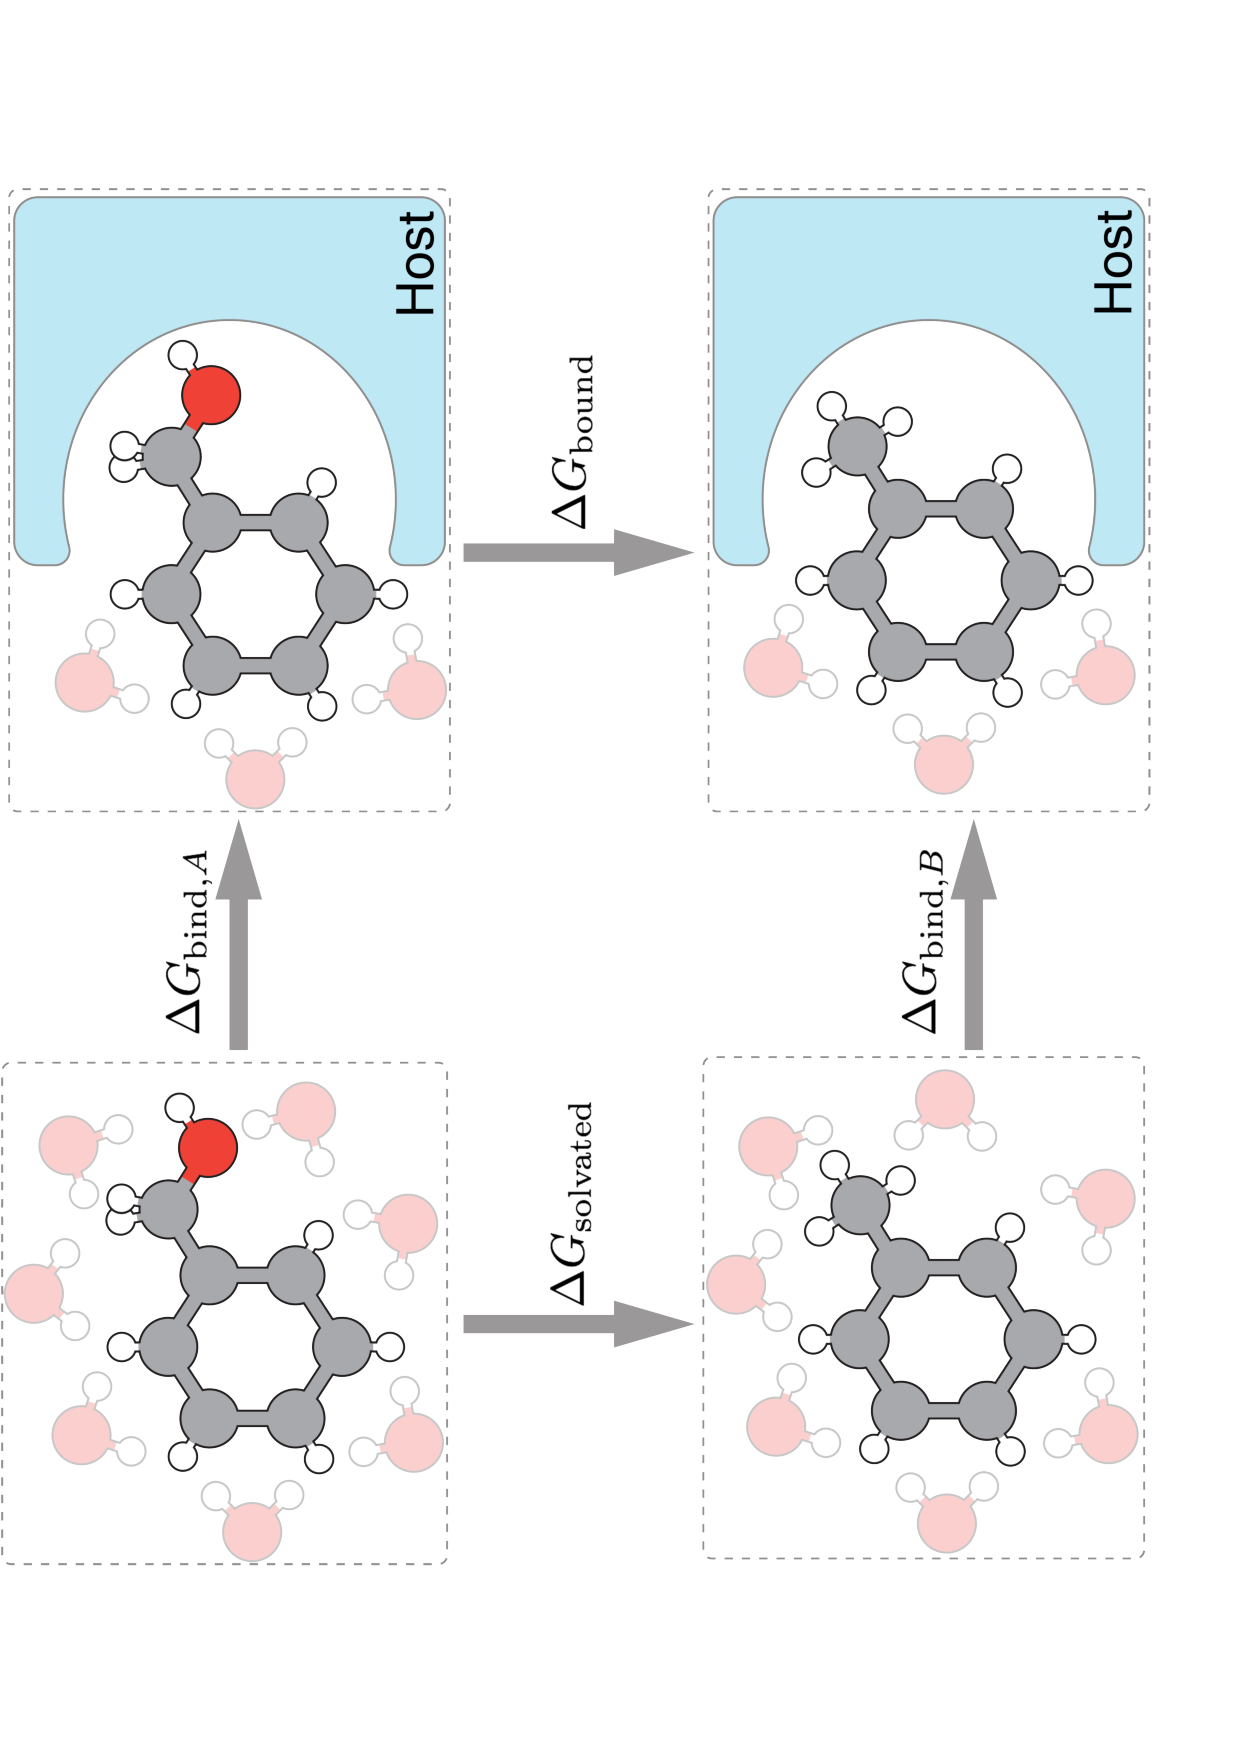
\includegraphics[width=0.95\linewidth]{paper/figures/fig2/Fig2.pdf}
    \caption{a) Bad alignment of congeneric series b) good alignment}
    \label{fig:fig1}
\end{figure}

If the binding site location is uncertain but the structure of the receptor is well defined and plausible binding sites are identified, you are more likely to chose an absolute free energy protocol to compute the standard free energy of binding of the ligand to a set of binding sites. This requires the user to prepare input files describing the bound conformation in different putative binding sites (REF). The apparent binding free energy of the ligand may be obtained by combining the individual binding site free energies, which also indicate where the ligand is more likely to bind. In this case using a docking program to generate initial structures is the way to go. Different commercial and none commercial tools are available, such as: rDock, Vina, glide, or Flare to name a few~\cite{rDock, Vina, Glide, Flare}. 
If the putative binding sites are not apparent because of for instance significant induced-fit effects it may be challenging to obtain meaningful free energies of binding. One would have to account for the free energy change for forming a binding site in the target receptor. However, it may still be possible to obtain useful binding free energy estimates that may be compared between different ligands.  

\subsection*{Free energies of hydration or partition coefficients}
Preliminary considerations necessary for using free energy methods to compute partition coefficients are much generally much more straight forward. Using even something such as bable to generate a 3D minimised structure of the solute you would like to compute a free energy of hydration or partition coefficient can be sufficient for preparation of these types of simulations. However, in these cases a careful choice of forcefields, as well as water models or organic solvents is essential. See for example XX.et al~\cite{xxx} for a good discussion on these choices. 
\todo[inline, color=green!20]{Just a note as a reminder: Chirality!}
%
%
%
%%%%%%%%%%%%
% Step 1   %
%%%%%%%%%%%%
%
\section{What simulation protocol should I choose? -- Step 2}
\label{sec:step2}
Alchemical free energy calculations can be grouped into two main categories, ``absolute'' and ``relative'' \footnote{The distinction is a bit of a misnomer, since both compute ratios of partition functions relative to another state, and neither computes an absolute free energy.}, which differ in whether they compute properties for a single molecule (absolute) or compare properties of different, usually closely related, molecules (relative).
To use binding as a concrete example, in absolute binding free energy calculations, one computes the binding free energy of a ligand to an individual receptor relative to a standard reference concentration.
In contrast, in relative binding free energy calculations, one compares the binding free energy of two related inhibitors to determine the potency difference.
\subsection*{Absolute and relative free energy calculations have some differences}
Many protocol issues for alchemical calculations are common, but some are different between absolute and relative calculations, so before treating the common elements we treat the protocol differences.
\todo[inline, color=green!20]{JM: single/dual hybrid toplogies what are they? ASJSM: These have been addressed below}



\subsubsection*{Choices unique to relative free energy calculations}

\paragraph{Topologies} A critical first step in relative calculations is to select an approach to these calculations, determining whether to use a \emph{dual topology}, \emph{single topology}, or \emph{hybrid topology} approach to relative calculations.
\begin{figure}
    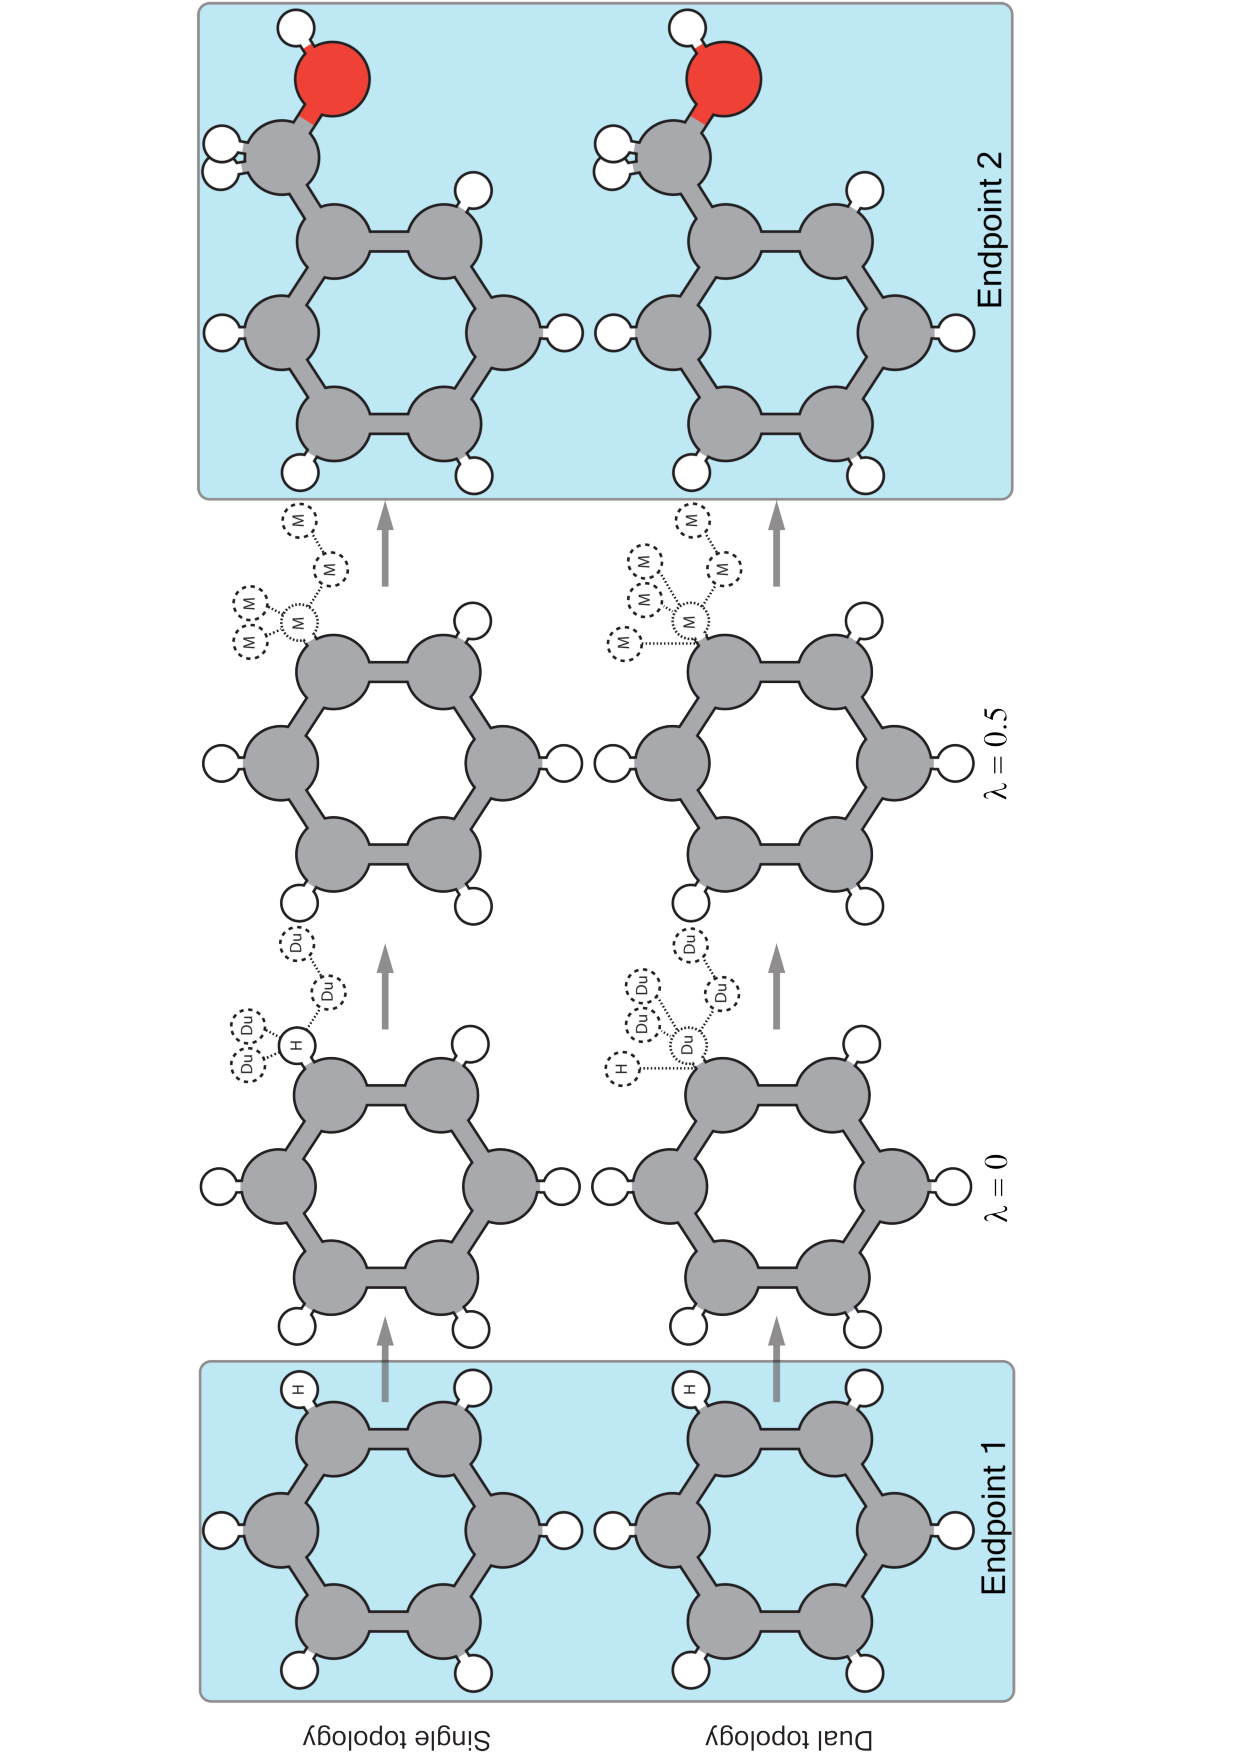
\includegraphics[width=0.95\linewidth]{paper/figures/fig4/topologies.pdf}
    \caption{a) single topology b) dual topology Figure adapted from \url{http://www.alchemistry.org/wiki/Constructing_a_Pathway_of_Intermediate_States}}
    \label{fig:topology}
\end{figure} 
The distinction between these can be illustrated by considering a hypothetical transformation from molecule A to molecule B, where both atoms share a common substructure but differ in which functional groups are present; e.g. consider a transformation of benzene (A) to benzyl alcohol (B)~\ref{fig:topology}.
In this case the common substructure is the benzene ring, though perhaps may be larger depending on how it is defined, as we discuss below.
In single topology calculations, the overall transformation is set up to involve as few additional atoms as possible, so benzene would be typically changed into benzyl alcohol by changing one of the hydrogens into a carbon. To this new carbon you also find non-interacting atoms called ``dummy atoms'' (retaining their bonded interactions but not interacting with the rest of the system), which will become the two hydrogens attached to the new carbon and the OH group. Bond parameters as well as partial charges are adjusted accordingly. 
Thus in a single topology calculation, atoms may change their type so relatively few dummy atoms are created. This is illustrated in fig.~\ref{fig:topology} (a). 
In contrast, in a dual topology free energy calculation, no atoms are allowed to change type~\cite{Shirts2012}. This means that the benzene to benzyl alcohol transformation involves starting with benzene plus the non-interacting dummy atoms making up the hydroxy methyl group, then passing through an intermediate state where atoms which are becoming dummy atoms or ceasing being dummy atoms are partially interacting (this state may or may not be well defined~\cite{Mobley:2014:J.Comput.AidedMol.Des.}  and culminating in a state where benzyl alcohol is present along with the additional dummy atoms which was previously a corresponding hydrogen of the benzene. Fig.~\ref{fig:topology} (b) depicts how such a dual topology works. 

Hybrid topology calculations have seen much less use but essentially consist of two absolute free energy calculations in opposite directions at the same time (turning one molecule off while turning the other on), and are best considered in that light~\cite{ [ref] }.
At present, the most widely used approaches, such as in Schrodinger's FEP+[ref] and in FESetup[ref] (for which calculations may be planned with Lead Optimization Mapper (LOMAP) [refs]) seem to use single topology approaches, though some codes only support dual topology.
To our knowledge efficiency differences have not been thoroughly explored, though conventional wisdom would suggest that fewer dummy atoms are better [ref LOMAP paper/Mobley perspective].

\paragraph{Atom mapping}
Once a particular approach to the topology is selected, a crucial next step is to identify the common atoms which will not be perturbed.
Rigorously, this process essentially comprises a maximal common substructure (MCSS) search of the molecules involved to identify the common substructure -- though the parameters of the MCSS search will differ depending on whether single or dual topology calculations are planned.
Specifically, with a single topology approach in mind, atom types are allowed to change, so a permissive MCSS search can be done, whereas with dual topology a more strict search is required.
\begin{figure}
    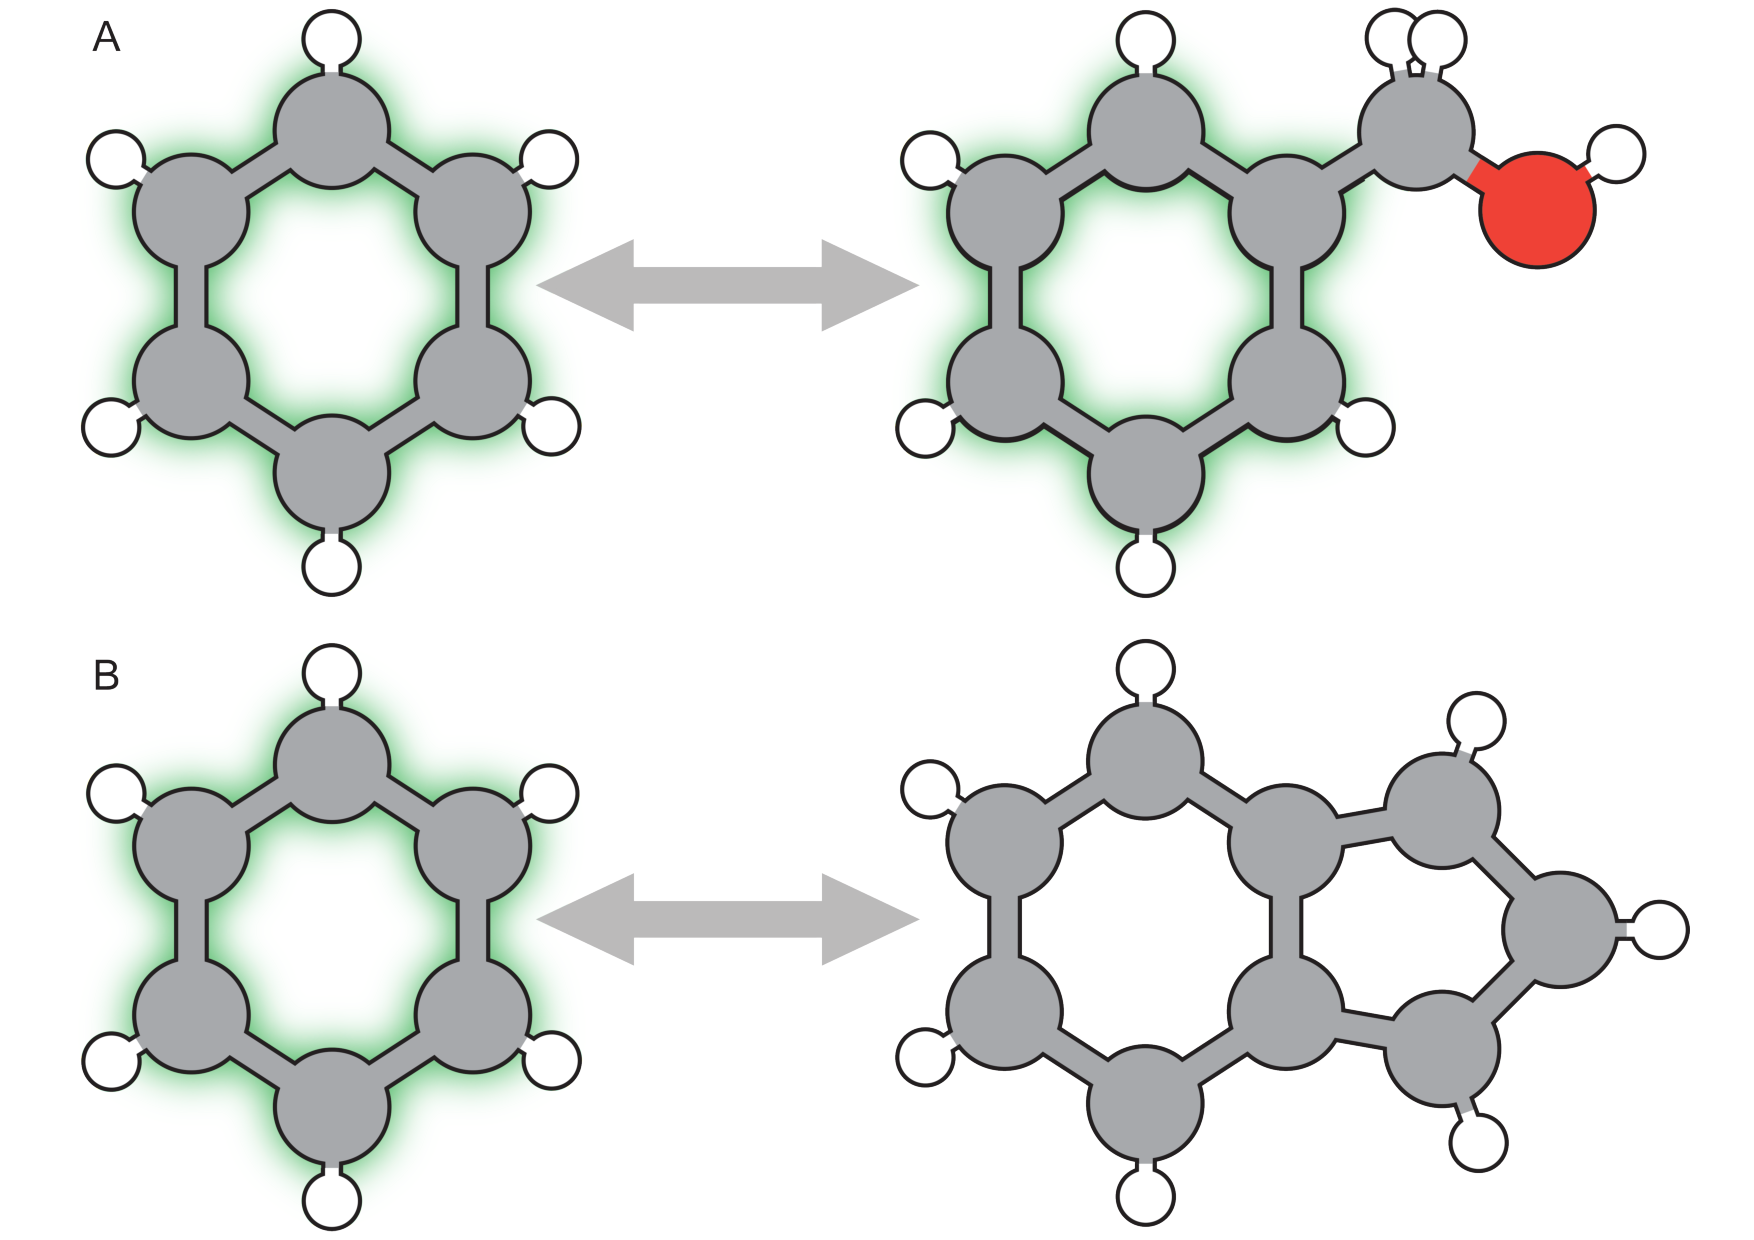
\includegraphics[width=0.95\linewidth]{paper/figures/fig5/MCS.pdf}
    \caption{a) restrictive MCSS match b) ring breaking}
    \label{fig:mcss}
\end{figure} 

There are different tools that allow the generation of MCSS matches as well as single topology input. A large number of software tools are nowadays available for computing MCSS matches, some of the rely on RDKit for this computation, such as LOMAP or FESetup and partially BioSimSpace, others such as fkckombu are standalone tools~\cite{rdkit, lomap, fesetup, biosimspace, fkcombu}. Schr\"{o}dinger's FEP+ planning tool is based on a version of LOMAP, also allows MCSS matching and planning single topology calculations between molecules~\cite{FEP+}. 

MCSS searches can be relatively time consuming, so if scoring a library of ligands to identify promising pairs for relative calculations is the goal, it can be helpful to use faster approaches such as shape similarity to perform an initial scoring and then use MCSS only to identify final mappings for relative calculations.

The MCSS approach, though relatively standard, takes into account only topological similarity.
It is possible that changes in binding mode could actually require a different choice of mapping, so in some cases mappings may need to be planned differently depending on 3D positioning of atoms in space [ref; does Cournia paper address this?].

Single topology relative calculations, and calculations based on substructure searches, only work if in fact the ligands share a common substructure, e.g. are part of a congeneric series.
If no common substructure is shared, then essentially one ends up needing sophisticated dual or hybrid topology free energy calculations, where one would co-localize a pair of compounds in a binding site, exclude their interactions with one another, and compute the relative binding free energy by turning one molecule on from being dummy atoms while turning the other off.
To our knowledge no general pipeline for such calculations yet exists and this would likely remain a research problem. Using an absolute style free energy calculation instead seems a more promising approach in such a case. 

\paragraph{Ring breaking and forming.} Relative free energy calculations for ring breaking and forming are particularly challenging/problematic, in part because relative calculations rely on the free energy contributions of dummy atoms canceling between different legs of the thermodynamic cycle [refs], which may not be true whenever dummy atoms are involved in rings.
Some approaches have attempted to address this [ref Schrodinger] but a general solution is not yet in mainstream use.

\paragraph{Perturbation maps}
As part of LOMAP and the FEP+ planning tool. Based on the input ligand series a perturbation map can be planned. Recent heuristics have shown the more connected the perturbation network the better, however there is away to optimise network structure while minimising the number of perturbations that need to be computed minimising the resulting computational cost~\cite{Mobely2019}. Sometimes the introduction of intermediates that are not part of the original congeneric series are essential to avoid ring breaking, or dealing with perturbations that would otherwise result in large numbers of atoms to be grown or disappearing. None commercial tools have underlying good heuristic but may fail with complicated input, needing user validation in particular when dealing with chiral compounds. 

\paragraph{Constraints and relative free energy calculations.}
One issue which requires particular care is the use of constraints.
Commonly, bonds involving hydrogen are constrained to a fixed length to allow the use of longer timesteps.
However, in single topology relative free energy calculations, the atoms involved might be mutated to other atom types -- for example, in a mutation of methane to methanol, one hydrogen might become an oxygen atom.
Typical molecular dynamics engines are not set up to recognize this change, or at least not to correctly include contributions to the free energy from changing constraints/constraint length, so results for a transformation would usually be erroneous.
At present the most general solution to this problem is simply to avoid the use of constraints (and thus use a smaller timestep if necessary, usually of around 1 fs) in any relative free energy calculation involving a transformation of a constrained bond.

\subsubsection*{Absolute free energy calculations must handle the standard state and use restraints}
\label{sec:standardstate-restraints}

\todo[inline, color={red!40}]{LNN: complete discussion about Boresch restraints}

\todo[inline, color={red!40}]{AR: would the explanation in the next paragraph be better suited for a more general section?}

\begin{figure}
    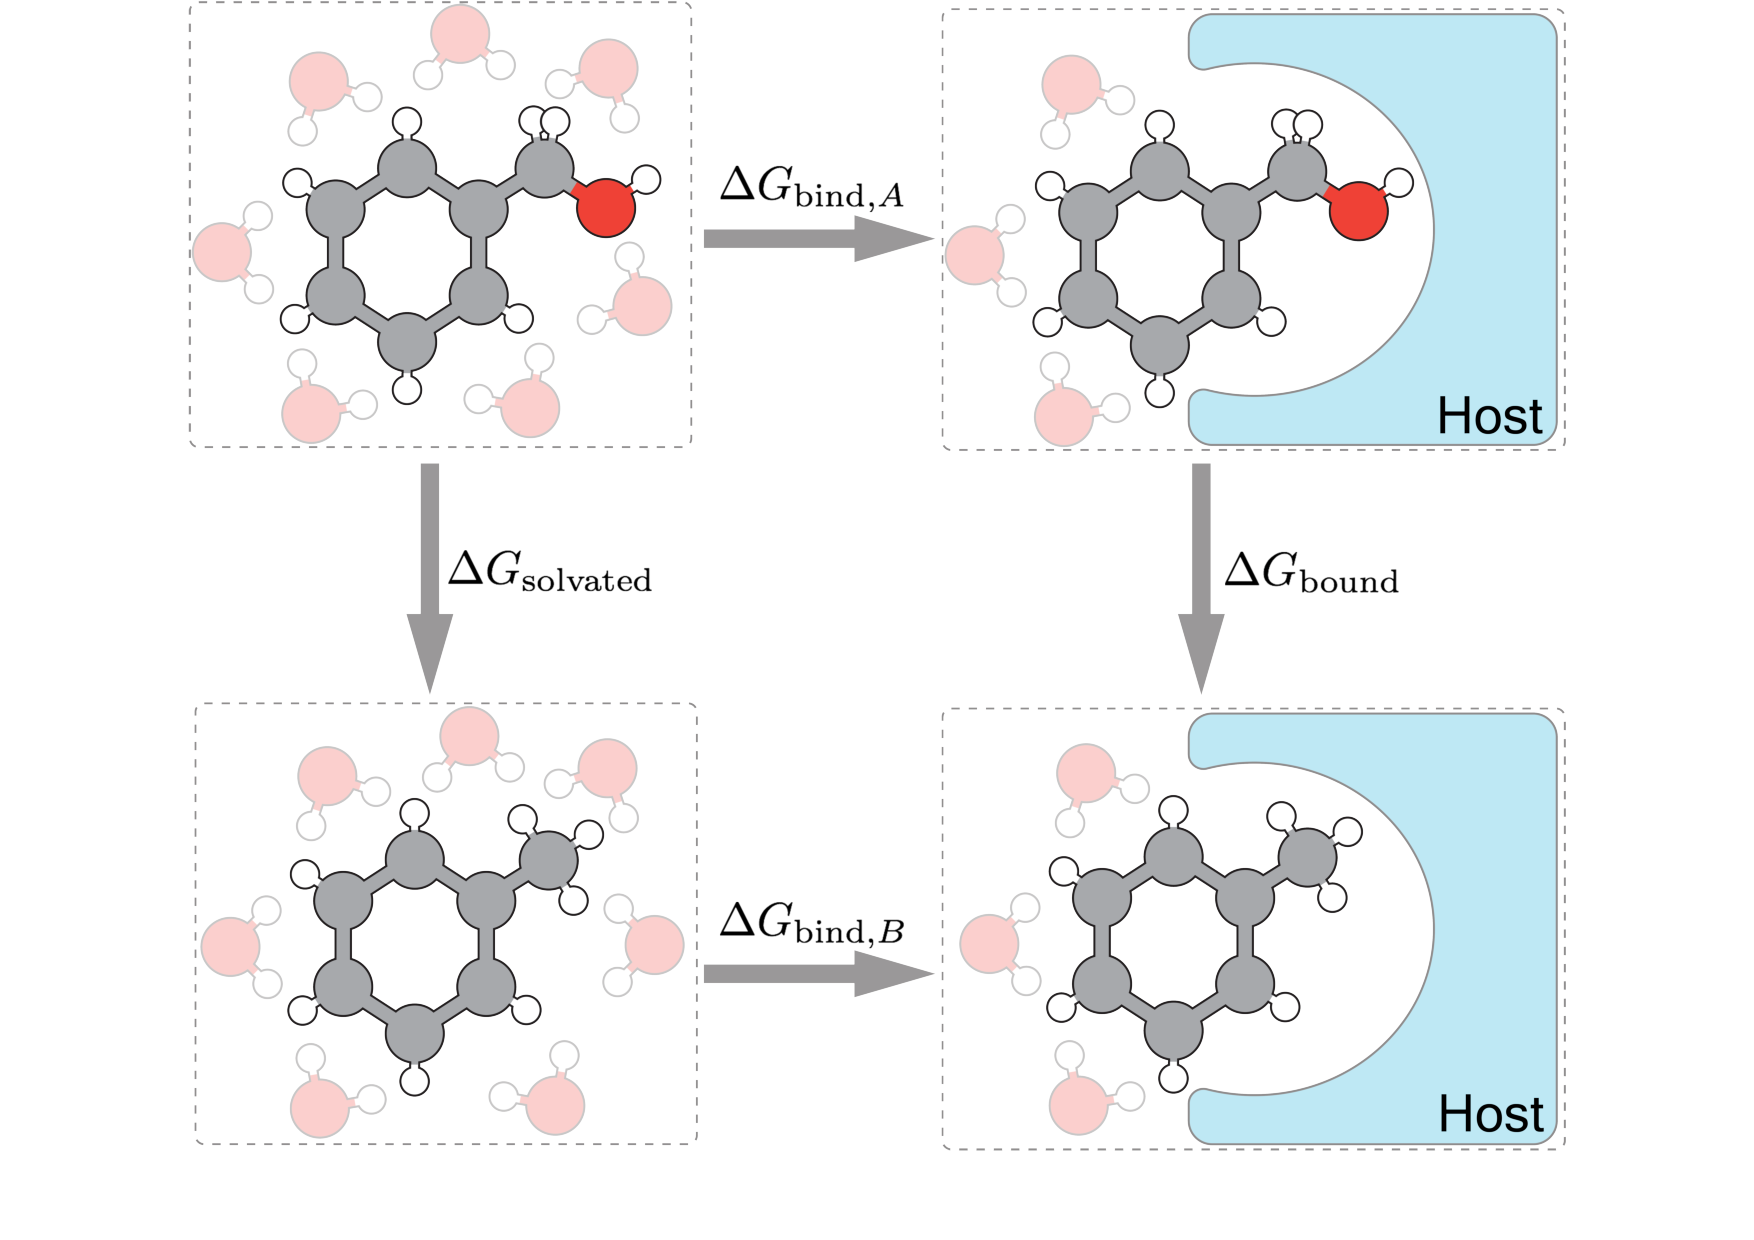
\includegraphics[width=0.95\linewidth]{paper/figures/fig6/Fig3.pdf}
    \caption{Absolute thermodynamic cycle}
    \label{fig:fig1}
\end{figure}

Absolute free energy calculations involve completely removing the interactions between the ligand or solute and its environment, taking it to a non-interacting state that may or may not retain intramolecular non-bonded interactions.
This non-interacting state can then be shifted between environments (from the protein to water, or from one solution to another) without changing its free energy, and then interactions can be restored.

Absolute free energies are typically reported with respect to a specific reference or standard state, which effectively determines the arbitrary point at which the free energy is 0.
The role of the standard state is particularly evident with binding free energies, in which having a reference state allows us to obtain a well-defined partial molar free energy for the reaction
\begin{equation*}
\ce{AB <=> A + B}
\end{equation*}
through the well-known expression derived from the law of mass action
\begin{equation} \label{eq:DGfromKAB}
\Delta G = -RT ~ \ln \left( C^0 K_{AB} \right)  = -RT ~ \ln\left( \frac{C^0 C_{AB}}{C_A C_B} \right) ,
\end{equation}
where $R$ is the gas, $T$ is the temperature, $C_X$ is the equilibrium concentration of the chemical species $X$ in the reaction solvent, and the reference state concentration $C^0$ converts the binding constant $K_{AB}$ into a dimensionless quantity expressed in reference concentration units.
It should be noted that ignoring the term $C^0$ is equivalent to assuming a reference concentration of 1~D$^{-1}$, where D are the units used to express $K_{AB}$, and would thus cause the value of $\Delta G$ to vary with the choice of the units.
Typically, it is convenient to define a standard state at a constant pressure of 1~atm and where each chemical species (i.e., A, B, and AB) in the reaction solvent has a concentration of $C^0$~=~1~M~=~1~molecule/1660~\r{A}$^3$ but do not interact with other molecules of A, B, or AB.

\paragraph{Handling the standard state in absolute free energy calculations.}

For solvation free energy calculations, handling the standard state is typically straightforward, and treating it correctly simply means ensuring that the non-interacting solute is taken to the same (or equivalent) final reference state in both environments, e.g. that the transformation involves a 1M to 1M equivalent transfer free energy (where the non-interacting solute still occupies essentially the same volume as the solute in the interacting system).
So typically in such cases no special care is required to ensure the correct standard state, as long as the \emph{experimental} data being analyzed uses the same standard state and if it does not, a simple entropic correction is needed.

However, for binding the situation is much more complex and requires special care.
Experimental absolute binding free energies are reported relative to a specific reference state -- a 1 M standard state -- which must also be used in calculations.
In practice, this has implications for how the calculations are done, as the reference concentration must enter the thermodynamic cycle employed.


Typically, to deal with both practical sampling issues and the standard state issue, restraints are employed in absolute binding free energy calculations to keep the ligand in a well defined volume as its interactions with the system are removed [ref Gilson 1997 BPJ].
This solves two problems.
First, if the ligand were not kept in a well-defined region, as its interactions were removed it might wander the system, perhaps quite slowly, and only inadequately sample the noninteracting or weakly interacting state -- yet adequate sampling of these states might be required for convergence.
So for practical purposes, the use of restraints can dramatically improve sampling as interactions are weakened and removed.
Second, if the ligand is not kept in a well-defined region then it is hard to determine how to link a computed binding free energy to the correct 1M standard state.
In contrast, with restraints, the free energy of releasing the restrained ligand to a 1M standard state can be computed analytically or numerically by solving the relevant integral [refs], allowing the standard state to enter the thermodynamic cycle [refs].

\paragraph{Several choices of restraints are possible.}
In practice, a variety of types of restraints are common, from simple harmonic distance restraints between the ligand and the protein [refs], to flat-bottom restraints which work similarly but only exert a force if the ligand leaves a specific region [refs].
\todo[inline, color={blue!20}]{DLM: Enlist Naden to discuss problems with analytical approximation to standard-state correction for Boresch restraints}
Alternatively, a set of restraints proposed by Boresch have also commonly been employed, where all six rigid-body degrees of freedom governing the orientation of the ligand relative to the receptor are restrained [refs].
Further restraints, such as on the overall ligand RMSD have also been used [ref Roux].

In principle, all of these forms will yield correct binding free energies in the limit of adequate sampling (if their effects and connection to the standard state are correctly handled) but they have different strengths and weaknesses.
For example, with more involved restraints, sampling at intermediate lambda values will not likely need to be as extensive but more computational effort must go to computing the restraining free energy.
Additionally, such restraints would typically keep the ligand from exploring alternative binding modes, which may be undesirable with Hamiltonian lambda exchange or expanded ensemble techniques where allowing the ligand to exchange binding modes when it is non-interacting could provide sampling benefits [refs, including Yank docs].
Concretely, flat bottom restraints might allow a ligand to explore multiple binding sites, harmonic restraints multiple binding modes within a site, and Boresch restraints a single binding mode within a single site [ref Yank docs?].
See additional discussion of the possibility of multiple binding modes below~\ref{sec:multiple_binding_modes}.

Many choices of restraints involve selecting reference atoms.
Again, in principle this choice is unimportant given adequate simulation time but practical considerations may be important.
The choice is likely especially important with Boresch-style restraints, where some relative placements of reference atoms are likely to be numerically unstable; additionally, ligand reference atoms should likely be in a part of the molecule which defines the binding orientation well, rather than in a floppy solvent-exposed tail, for example.
\todo[inline, color={blue!20}]{DLM: Get input from JDC on what they've learned about these.}

\todo[inline, color={blue!20}]{DLM: Clarify terminology: Double decoupling, etc. See Feature Box below.}


\subsection*{Absolute and relative calculations must deal with some of the same issues}

\subsubsection*{Structural definition of the bound state and weak binders}

In binding free energy calculations, extra care should be taken when simulating the bound state, especially when dealing with weak binders and absolute free energy calculations in combination with enhanced sampling techniques.
In principle, only configurations of the receptor-ligand complex that we consider "bound" should be sampled from the bound state, and, in atomistic simulations, this requires to establish a structural definition of the bound state.
In practice, the simulation of the bound state starts with the ligand already placed in the binding site and relies on kinetic trapping to maintain a bound complex.
However, this strategy may not be sufficient if the complex dissociation rate is high or if methodologies such as Hamiltonian replica exchange [ref] and expanded ensemble [ref] are employed in absolute free energy calculations to enhance sampling since, in both cases, the ligand may find a way out of the binding site on timescales that are achievable by modern MD simulations.
A solution commonly adopted in these cases is the use of one or more restraints making the unbound configurations energetically unfavorable through the addition of extra terms in the potential function.
In practice, even with restraints, it is not always trivial to force a molecular dynamics simulation to explore a restricted region of the configurational space with a complicated geometry such as a binding site.
If the ligand is a tight binder\todo[inline, color={red!40}]{AR: Should we give an order of magnitude to define a tight and a weak binder?}, it is usually safe to employ a restraint that allows some of the unbound configurations to be sampled since they generally contribute negligibly to the partition function (i.e., they have a relatively small Boltzmann weight) as long as the sampled volume is not so large that their cumulative contribution becomes significant.
However, this is more problematic when dealing with weak binders as the unbound configurations can have a non-negligible Boltzmann weight, and their binding affinity can exhibit a significant dependency on the restraint type and parameters that are used to determine the sampled volume [ref].
Moreover, it should be noted that the additional potential energy terms used to model the restraints can introduce a bias in the predicted free energy.
The bias can be removed at the analysis stage through reweighting techniques, but this procedure can increase the statistical uncertainty of the binding free energy estimate when the restraints are so strong that the overlap with the reweighted state is diminished [ref].

Finally, it is useful to keep in mind that, for a meaningful comparison between computational predictions and experimental measurements, the definition of the bound state should be consistent.
In particular, this means that the signal used by the experimental methodology to determine the fraction of bound complexes in solution should in principle reflect the population of complexes in the bound state as defined in the calculation.

\subsubsection{Changes in net charge can be challenging/problematic.}

If the net charge of the system will change as the alchemical calculation progresses, this can pose major challenges.
Specifically, finite-size effects can introduce profound artifacts into computed binding free energies [refs], in part because typical schemes for long-range electrostatics (including PME and reaction field) do not handle free energy contributions from such changes effectively or as they would be handled in a hypothetical macroscopic bulk solution [refs].

There are two main potential solutions to avoid artifacts due to changes in net charge: Correcting for the introduced artifacts, or avoiding changing the net charge.

Many relative free energy planning tools have been set up to avoid changing the net charge of the systems considered, including LOMAP [ref] and early implementation of Schr\"{o}dinger's FEP+, though later implementations allow changes in net charge by including charge corrections.

Absolute free energy calculations can potentially avoid changing the charge of the system by making a charge perturbation of equal and opposite sign elsewhere in the system; for example, as a charged ligand is removed, a charged counterion of opposite sign could also be removed, or one of the same sign could be inserted.
This is the approach employed by the Yank free energy package [ref].

Charge corrections have also been explored, and are potentially a viable solution to this problem [refs] where artifacts introduced by finite-size effects are corrected numerically.
However, application of such corrections typically remains a research problem (except in the FEP+ protocol [ref]).

When free energy calculations \emph{do} need to change the charge of a ligand or solute, the literature does not yet seem to indicate what approach should be preferable, so considerable care should be taken.
We are not yet aware of a careful comparison of charge corrections versus other approaches such as decoupling an ion at the same time, so in our view the issue of proper handling of charge mutations in the context of alchemical calculations remains a research problem.

\subsubsection*{The alchemical pathway is quite important \label{sec:important_path}}

\todo[inline, color={red!40}]{LNN: write common principles alchemical path choice}
\todo[inline, color={red!40}]{AR: write absolute-specific section on  alchemical path choice}
\todo[inline, color={red!40}]{BA: write relative-specific section on  alchemical path choice}

Both absolute and relative calculations must choose an alchemical pathway connecting initial and final states, which is in principle arbitrary but in practice affects the efficiency of the calculations considerably.
Some choices are particularly crucial -- for example, transformations involving insertions or deletions of atoms should employ soft-core potentials for Lennard-Jones or other hard-core interactions [refs].
Other issues, such as whether absolute calculations retain intramolecular nonbonded interactions or remove these interactions, may be less critical and differ among studies in the literature [refs].

Relative calculations introduce additional choices, including whether to define explicit intermediate states [ref] or leave these implicitly defined by the code [ref].
Typically in single topology relative calculations it proves most efficient to first remove electrostatic interactions of any atoms which will be deleted, then modify other nonbonded interactions, then restore electrostatic interactions of any atoms which are being inserted.
Other schemes, such as simultaneously changing electrostatic and Lennard-Jones interactions, even with electrostatic ``soft core'' potentials, in our experience typically introduce errors and/or instabilities or are at least unreliable.
We have less experience with dual topology calculations but expect that similar considerations will apply, and the principle of first removing electrostatics and then removing steric interactions will likely serve well.

A key additional consideration in choosing the alchemical pathway is the choice of spacing of intermediate states.
The spacing depends to some extent on the choice of analysis method, though states should essentially be spaced equidistant in the relevant thermodynamic length [ref].
For BAR/MBAR techniques this means that spacings should typically be equal in [what, variance? ref].
Some schemes to adaptively optimize the spacing of intermediate states based on initial exploratory simulations have been proposed [refs].

An example of this approach for relative binding free energy calculations includes saving configurations from short 10 picosecond simulations starting at $\lambda_0$, and evaluating changes in the standard error of mean (SEM) in $\frac{dU}{d\lambda}$ as reevaluated at new values of $\lambda$, starting with a step size of 0.01 up to a predetermined threshold.
This threshold can be empirically defined as the number of atoms being inserted or deleted in the simulation / 100.
If the absolute value of the difference in SEM is below the defined threshold, then the change in $\lambda$ for re-evaluation of SEM in $\frac{dU}{d\lambda}$ is defined by the current difference in SEM from the threshold divided by the derivative of the SEM with respect to $\lambda$.

\begin{enumerate}

\item Choice of discrete alchemical protocol (Shirts, Mey, Chodera)
	%\begin{itemize}
	%\item Many options: Adaptive scheme, Chebyshev polynomials, linear spacing, ``choose your next lambda from data at this lambda'' ��, optimal thermodynamic length approaches (separately: Shirts, Sivak, Huafeng Xu).
	%\item Levi Naden had paper with lambda protocol which worked for all cases -- methane solvation, host-guest (including disappearing host)
	%\end{itemize}
\item Relative
Three-stage protocol (discharge unique initial atoms, transform LJ, charge unique final atoms) vs softcore electrostatics/LJ

\item Absolute
	\begin{itemize}
	\item Select a \textbf{common alchemically-eliminated end state}
	\item Decoupled vs annihilated for electrostatics and LJ
	\item Sequential electrostatics and LJ versus simultaneous (recommend sequential)

\end{itemize}
\item Concerns:
Part of AMBER still can’t run at endpoints (lambda = 0 or 1); SANDER cannot but PMEMD can.

\end{enumerate}


\subsubsection{Multiple or uncertain binding modes may require considerable care}
\label{sec:multiple_binding_modes}

In a discovery setting, new ligands typically have unknown or at least uncertain binding modes~\cite{Kaus:2015:J.Chem.TheoryComput., PlountPrice:2000:J.Am.Chem.Soc.} [refs, including Mobley Structure paper and recent paper on non-additivity], complicating binding free energy estimation.
This uncertainty is because it is usually not desirable to estimate a binding affinity for a ligand which already has an available bound structure, since such a compound has already been tested.
To deal with prospective ligands with unknown binding modes, discovery projects commonly assume that modifications of functional groups on a common scaffold result in a consistent binding mode across all members of a series.
This is not necessarily always the case~\cite{Kaus:2015:J.Chem.TheoryComput.}, as reviewed elsewhere [ref Mobley Structure paper] and in some cases unexpected binding mode changes can be the origin of apparent non-additivity in structure-activity relationships [ref non-additivity paper].
Binding modes also tend to be particularly variable in the case of fragments, which often may have multiple relevant binding modes [refs].

Absolute free energy calculations for dissimilar ligands can have particular challenges with binding modes, because the (potentially incorrect) assumption of consistent binding modes across a series of similar ligands provides even less help in this case.
This means that researchers performing absolute binding free energy calculations will have to pay particular attention to generating reasonable putative binding modes.

In some cases, it is tempting to simply use docking techniques to generate initial bound structures for starting molecular dynamics simulations.
However, timescales for binding mode interconversion are usually slow compared to MD/free energy timescales, meaning that simulations started from different potential binding modes are likely to yield disparate computed binding free energies~\cite{Mobley:2006:TheJournalofChemicalPhysics, Palma:2012:J.Comput.Chem., Mobley:2012:TheJournalofChemicalPhysics, Gill:2018:J.Phys.Chem.B} .
And docking techniques are good at identifying sterically reasonable potential binding modes, but still perform relatively poorly at identifying a single dominant binding mode \emph{a priori}. [refs] 

It is worth highlighting a recent SAMPL blind challenge on HIV integrase as an illustration of this. 
Many submissions, using state-of-the-art methods, had difficulty even predicting which \emph{binding site} ligands would bind in (most submissions placed more than half of the ligands into the incorrect binding site), and even given correct binding sites, the binding mode within each site was also quite difficult to predict~\cite{Mobley:2014:J.Comput.AidedMol.Des.}.
The best performing submission for predicting binding modes actually ended up being a human expert (aided by computational tools) with more than 10 years of experience on the particular target~\cite{Voet:2014:JournalofComputer-AidedMolecularDesign}, rather than a fully automated approach.
While free energy calculations on this set had some success, many of the failures actually ended up being cases where the binding mode selected as input for free energy calculations was later found to be incorrect~\cite{Gallicchio:2014:JournalofComputer-AidedMolecularDesign}, highlighting the importance of these issues.

One approach which has shown some success is to retain diverse potential binding modes from docking, perform short MD simulations of these to identify distinct stable binding modes, and then consider these in subsequent calculations~\cite{Gallicchio:2014:JournalofComputer-AidedMolecularDesign, Mobley:2006:TheJournalofChemicalPhysics, Rocklin:2013:JournalofMolecularBiology, Boyce:2009:JournalofMolecularBiology, Mobley:2007:JournalofMolecularBiology}.

Routes to handle multiple potential binding modes are different depending on whether absolute or relative calculations are selected, unless a method is available to estimate the relative populations of different stable binding modes in advance (e.g. such as the BLUES approach currently in development~\cite{Gill:2018:J.Phys.Chem.B}), in which case this approach could be applied to assist both types of calculations.



\paragraph{Handling multiple potential binding modes within absolute calculations.}
Within absolute binding free energy calculations, multiple potential binding modes can be handled by two main strategies: Consider each binding mode separately (a separation of states strategy) or sample all binding modes within a single simulation~\cite{Mobley:2012:TheJournalofChemicalPhysics}.
This couples to the choice of restraints selected, as some restraints will allow transitions between binding modes and even binding sites (Section~\ref{sec:standardstate-restraints}), and others do not.

Sampling all binding modes within a single free energy calculation is usually impractical without some form of enhanced sampling or at least Hamiltonian replica exchange~\cite{Wang:2013:JournalofComputer-AidedMolecularDesign} because barriers for binding mode interconversion result in kinetics which are too slow compared to simulation timescales~\cite{Mobley:2006:TheJournalofChemicalPhysics, Palma:2012:J.Comput.Chem., Mobley:2012:TheJournalofChemicalPhysics, Gill:2018:J.Phys.Chem.B}.
Hamiltonian exchange, coupled with appropriate restraints, can allow the ligand to relatively rapidly exchange between potential binding modes when non-interacting, accelerating sampling of binding modes~\cite{Wang:2013:JournalofComputer-AidedMolecularDesign}.
\todo[inline, color={yellow!40}]{DLM probably need more background refs on Hamiltonian lambda exchange here.}

Separation of states provides a simple though potentially expensive alternative, where each stable binding mode is considered separately with a binding free energy calculation restricted to that binding mode, and then (as long as the binding modes are non-overlapping) the resulting component binding free energies can be combined into a total~\cite{Mobley:2006:TheJournalofChemicalPhysics, Mobley:2012:TheJournalofChemicalPhysics}.
This approach necessitates a separate binding free energy calculation for each potential binding mode, however, so it can be computationally quite costly.
If relative populations of different stable binding modes were available from some other technique, it could make this separation of states approach considerably more efficient~\cite{Mobley:2012:TheJournalofChemicalPhysics, Gill:2018:J.Phys.Chem.B}.

\paragraph{Handling multiple potential binding modes within relative calculations.}

Multiple potential binding modes pose particular problems for relative free energy calculations, as having multiple starting structures for these calculations could yield substantially different calculated relative binding free energies for the same transformation due to kinetic trapping, and, without additional information (specifically, the free energy of binding mode interconversion or, equivalently, the relative populations of different binding modes) it becomes impossible to sort out which of the multiple answers is in fact the correct relative binding free energy [refs].

To deal with this, some practitioners have actually computed relative binding free energies of different binding modes of the same ligand~\cite{Palma:2012:J.Comput.Chem.} [ref Jorgensen (?) etc.].
For example, a mutation which adds a methyl to an aromatic ring of a larger ligand might yield one result if the methyl points in one direction, and a different value if it points in the other due to slow ring motions. [e.g. get ref from Sukanya]
One could compute the free energy of turning off the methyl group in one orientation and turning it back on in the other orientation to obtain the free energy difference between the two potential binding modes.
While this approach has precedent, it is relatively difficult to automate at present and requires considerable care.

Overall, this likely means that relative free energy calculations will be susceptible to problems resulting from uncertainty in ligand binding modes until more robust approaches are available to determine dominant binding modes, or the relative populations of different potential binding modes, in advance.


\subsubsection*{How long should I run my simulation for and what information should be saved?}

% \todo[inline, color={red!40}]{LNN, BA: write stopping condition section}
% \begin{enumerate}
% \item Determine \textbf{stopping conditions}
% Uncertainty-directed stopping criteria can ensure target uncertainty is achieved


% \item Select which \textbf{data should be saved and with which frequency}
% \begin{itemize}
% \item What data to save: dU/dlambda, Delta E’s between neighbor for BAR, between further for MBAR, …
% \item BAR captures most of info with well-optimized lambda protocol, but MBAR when perhaps not, except when there are way too many lambda values.
% \item Recommend against solely relying on TI when possible
% \item Recommend cross-comparing methods (TI (spline, trapezoid, etc.), BAR, MBAR) as diagnosis of trouble
% \end{itemize}
% 
% \end{enumerate}

The conditions on when to stop alchemical free energy calculations should be determined before they are started, and the process of detecting whetn the calculation should be stopped may require several iterative checks. 
A metric of convergence should be chosen ahead of time to determine when the calculation should be terminated.
One useful metric is the target uncertainty of a desired free energy estimate, though care must be exercised should the uncertainty estimate prove unreliable.
In particular, if the rate of change in the free energy estimate is significant when this condition is met, the simulation may not be locally converged, and more sampling may be necessary to determine a stable free energy estimate which is no longer changing significantly over time. 
However, this is not the only metric which should be used, as the uncertainty only captures the information about the sampled phase space, not necessarily the entirety of the phase space.  
For example, 
convergence of relative free energy calculations in predictive simulations where the entire phase space not known in advance, requires sampling the different kinetically stable states \todo[inline]{cite Mobley and Klimovich JCP 2012}. 
This highlights the importance of choosing the correct thermodynamic path to ensure you sample the required thermodynamic states as discussed in Section~\ref{sec:important_path}.

The condition of minimizing the statistical uncertainty of different free energy estimators below a sufficient threshold should be one metric monitored over the simulation. This can be done through the uncertainty estimator built into certain analysis tools such as MBAR, or can be done though more general statistical tools like Bootstrap Sampling. 
A target statistical uncertainty should be chosen at the onset of the simulation to avoid excessively long simulations, or falling into the trap of running until the free energy estimate is "good enough," which is subjective and has no defined criteria. This could be a fixed value such as $0.20 \mathrm{kcal/mol}$, or a functional quantity such as "below $0.5 \mathrm{kcal/mol}$ and $10\%$ of the free energy estimate." The user does not need to monitor this information in real-time and can choose to run simulations for fixed duration (either time or number of samples) and run analysis on the data collected thus far. If more samples are needed, the simulations can be resumed, or, started again in different initial conditions. 

Convergence in other alchemical observables should also be monitored to determine if the defined phase space has been sufficiently sampled and enough decorrelated samples have been drawn. These additional observables include, but are not
limited to, the variance in $\frac{dU}{d\lambda}$ across all $\lambda$ values, calculating the variance in free energy using bootstrap analysis, and comparing differences in free energies calculated using different percentages of the simulation in both the forward and reverse directions (figure \ref{fig:convergence_forward_reverse}).

\begin{figure}
    \centering
    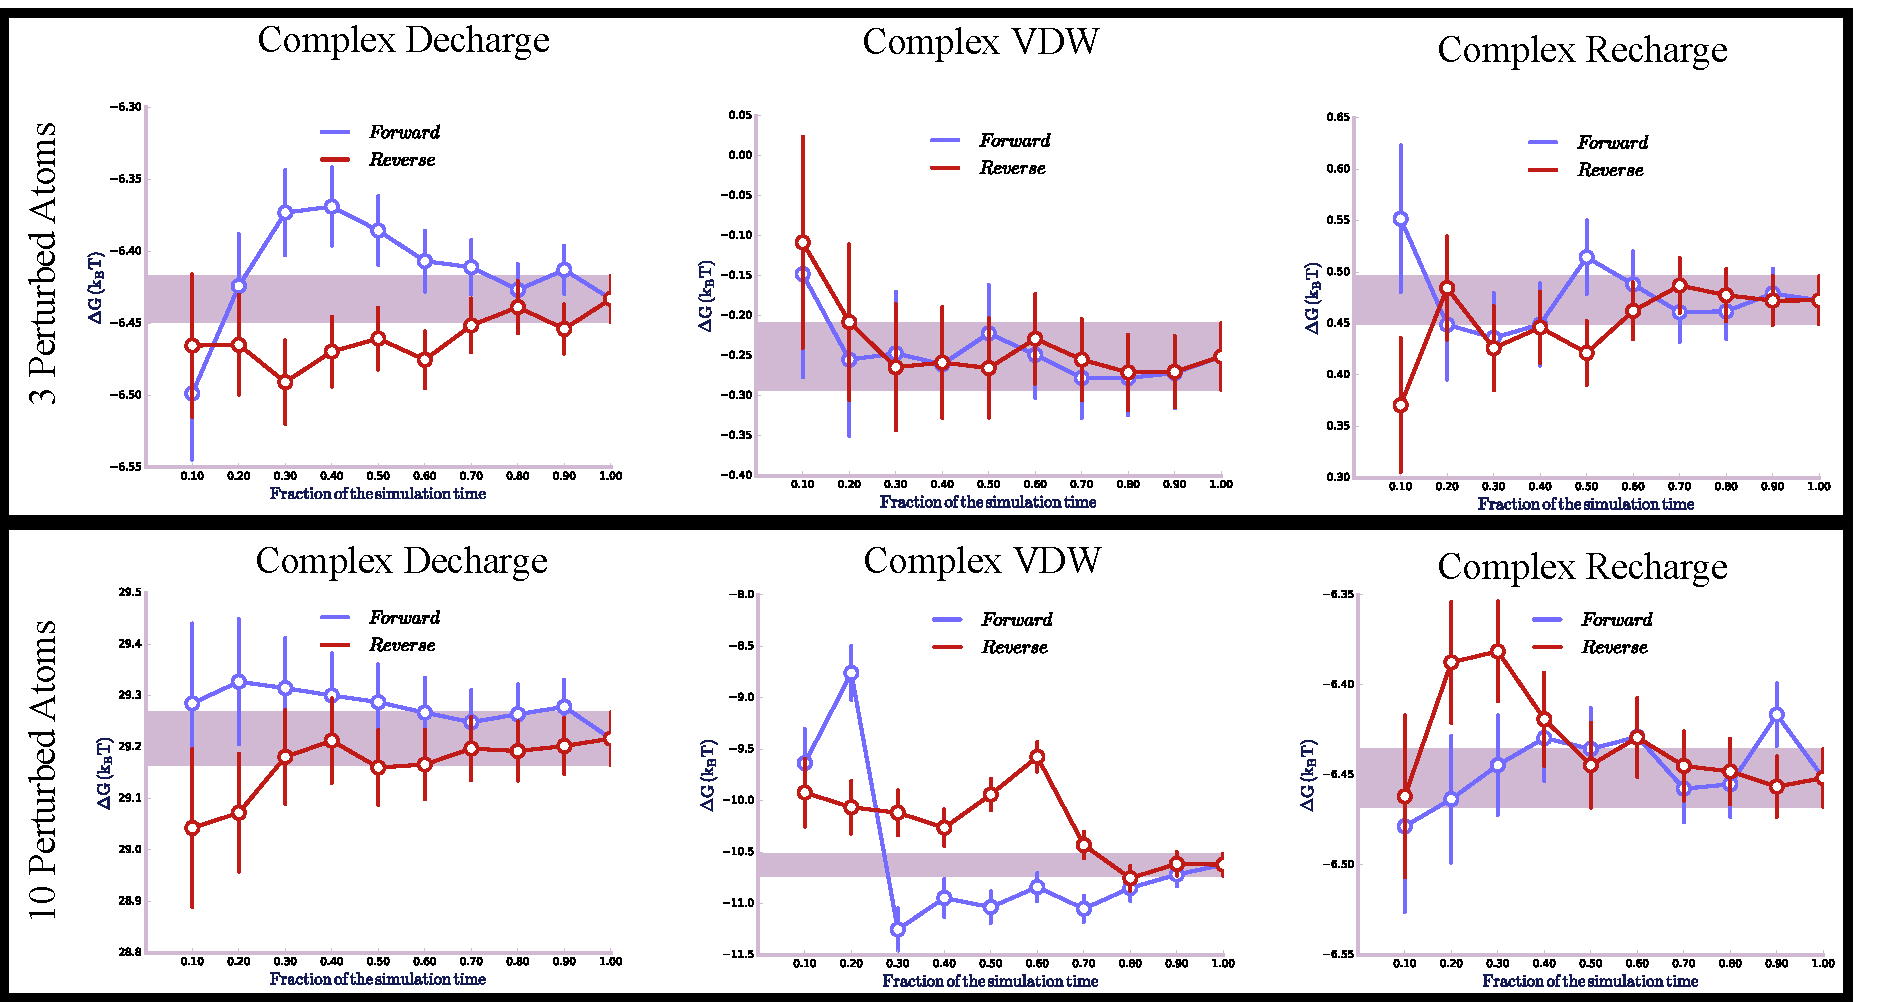
\includegraphics[width=0.95\linewidth]{paper/figures/figX/Forward_Reverse_Fig.pdf}
    \caption{Free energy (in k$_{B}$T) for two different relative binding free energy (RBFE) perturbations. 
    Each plot shows the estimated free energy change using a varying fraction of total simulation time (up to 5 ns total). 
    The top panel shows the three-step protocol for a perturbation involving 5 perturbed atoms, while the bottom panel shows the same protocol for a perturbation involving 10 perturbed atoms. The difference in energy between the forward (blue) and reverse (red) free energy calculations at the midpoint of the simulation time gives an indication of the overall convergence of the simulation, with differences over 1 k$_{B}$T indicating poor convergence.}
    \label{fig:convergence_forward_reverse}
\end{figure}

Each of these metrics have demonstrated promising results for diagnosing when a simulation has a convergence issue beyond simple convergence of uncertainty estimate. 
Results obtained from calculations with convergence issues should be checked for errors or run for longer before any confidence should be placed in conclusions drawn from their analysis.
In relative calculations that share similar binding modes, for example, and do not induce large conformational changes when in complex with protein, the need to sample exhaustively to converge estimates in free energy differences is often not necessary due to the locality of sampling changes in the molecular topology and shared phase space of the core atoms.
However, even subtly induced changes in protein binding configuration will require more sampling or cause local convergence to a free energy estimate that has high error.
Many enhanced sampling techniques have been proposed to try and overcome barriers in free energy calculations and mitigate convergence to erroneous estimates [ref]. 
The confidence a user should have in a free energy estimate is significantly improved when both the uncertainty of the free energy estimate is low, and when other observables have reached a convergence.

A simple, but effective, way of checking for convergence is to compute the same property by multiple estimators. 
The uncertainty in the free energy, for example, has multiple ways to be estimated, e.g. through MBAR's estimator, through bootstrap, through multiple runs, etc. 
Independent of how the property is estimated, its important to remember that they are \textit{estimations of the property}, not the true underlying property itself. 
These estimators are usually consistent estimators, not necessarily unbiased ones though.
As such, it is a good idea to subject different estimators to the same data to see if they yield either the same estimate (within error and bias), or if they fluctuate wildly. 
This is not a perfect method as some estimators, such as Exponential Averaging, will converge significantly slower, or never, relative to more accurate estimators like MBAR. 
Therefore, it is a good idea to subject the estimators to different fractions of the data to see if the main estimator of free energy you have chosen is stable.


The determination of what information to collect during the simulation is paramount to its success. If, for instance, the free energy estimator selected is Thermodynamic Integration, but $\frac{dU}{d\lambda}$ information is not collected, then no amount of simulation time will provide a means to estimate the free energy. Once a combination of knowing what type of simulation you will run, which alchemical topology you will simulate, what alchemical path you will simulation along, and what your stopping conditions are, then you are ready to enumerate the information you should capture. Below is a sample of the minimal information you need for a set of common estimators:

\begin{itemize}
    \item Thermodynamic Integration (TI) requires $\frac{\partial U(\vec{x})}{\partial\lambda}$.
    \item Exponential Averaging (EXP) needs \textit{either} $\Delta U_{k,k+1}(\vec{x})$ or $\Delta U_{k,k-1}(\vec{x})$, depending on the direction its being evaluated in.
    \item Bennett Acceptance Ratio (BAR) needs \textit{both} $\Delta U_{k,k+1}(\vec{x})$ and $\Delta U_{k,k-1}(\vec{x})$.
    \item Weighted Histogram Analysis Method (WHAM) and Multistate Bennett Acceptance Ratio (MBAR) both need the complete set of $\Delta U_{k,j} \, \forall \, j=\{1...K\}$. WHAM must have this information binned.
\end{itemize}

The potential derivative required for TI must generally be calculated during the simulation; it cannot be postprocessed by a code that does not evaluate the derivatives. 
If that option is unavailable, you can estimate it through finite difference (if sufficient information is collected), but understand this will introduce error and the BAR estimator may be a better, and simpler choice at that point as you will have at least the same level of information. 
The potential energy differences required for EXP, BAR, MBAR, and WHAM can be calculated either during the simulation or in post-processing. It is recommended to calculate the potential differences in code when possible to avoid extra overhead and possible errors produced by running the simulation twice, and to reduce the amount of stored information. 
Although TI must be usually be calculated in code, as it requires the derivative, there is one condition under which it actually has the fastest computation time. 
If the alchemical path you have chosen is a linear alchemical path, then you get $\frac{dU}{d\lambda} = U_0(\vec{x}) - U_1(\vec{x})$, which is the difference between the initial and final states. 
However, because of the problems with linear paths, this simplification is rarely that useful.

Free energy information should be saved as frequently as coordinate data, if not more frequently. 
The on-disk size of the data for free energy estimation is often significantly smaller than full atomic coordinates, so the information should be collected at least as frequently, if not more. 
However, the information should not be collected \textit{every} time step, as most free energy techniques are operated at equilibrium, and need equilibrated \textit{and decorrelated} samples for an unbiased estimate.
A sample collected every time step will likely result in most samples being discarded due to decorrelation routines in the analysis. However, if it is computationally cheap and disk space is plentiful, do save often. 
How decorelation impacts calculations, and how to compute it is discussed in other sections. [section ref]

\section{Step 3 -- Overview of available analysis techniques}
\label{sec:step3}
\todo[inline, color={red!40}]{JDC, BA: uncertainty estimation section}
\begin{enumerate}

\item Detecting boundary between equilibrated and production regions (Chodera: \url{http://dx.doi.org/10.1021/acs.jctc.5b00784})
\item Decorrelating samples for analysis
\todo[inline]{JDC: write section}
\begin{itemize}
\item Subsample different lambdas based on correlation times
\item Ensure all simulations at least 50x correlation time
\end{itemize}
\todo[inline]{MS: write section}

\todo[inline]{MS/JDC: write section}
\item Free energy differences between two different states differing in the energy function are directly related to the
ratio of probabilities of those states.AS can be noted, the partition functions in Eq.~\ref{equation:dimensionless-free-energy-difference} are simply the total accumulated probabilites for all possible configurations of the system. Virtually all of the ways to estimate this free energy are based in converting this ratio of integrals to something that can be measures in one (or several) simulations.  

\begin{itemize}
    \item \textbf{The Zwanzig relationship} Perhaps the simplest method for calculating free energy
differences from simulations is the so-called \textit{Zwanzig
relationship}~\cite{orig.TPT}, also called EXP or simply free energy perturbation, thought that term later grew to encompass all ways of calculating free energy differences.
The free energy between two states defined by two different potential energy functions 
$U_0(\vec{q})$ and $U_1(\vec{q})$ over coordinate space $\vec{q}$ can be calculated as:
\begin{eqnarray}
\Delta f_{01} & = & \ln \expect{e^{-(U_1(\vec{q}) - U_0(\vec{q}))}}_0 =  \ln \expect{e^{-\Delta U(\vec{q})} }_0
\end{eqnarray}\label{eqn.zwanzig}
In words, we take the samples generated during our run with the potential energy function $U_0(\vec{q})$, recalculate what the energy difference would be to switch to potential energy function $U_1(\vec{q})$, and exponentially average them to get the free energy.  Here, the exponential average consists in multiplying by -1, exponentiating, averaging, taking the logarithm, and multiplying by -1 again.  This almost requires no extra code functionality to perform; one need only to save a full precision trajectory, and run an unmodified molecular simulation code using the $U_1$ in order to calculate the new energies.  The analysis can be written in a line of code.  We note that this method is even more general, in that the instantaneous work to change the potential energy function from $U_0$ to $U_1$ can be replaced by the non-reversible work $W$ to make the same change some conditions~\cite{xx} 
Although the Zwanzig equation is formally correct (as long as the two states considered sample the same phase space volume), it has some very important numerical issues that mean that it is usually when performing a standard free energy calculation for a small molecule.~\cite{shirts.comparison,LuND:Appmcf}  One can show that if the standard deviation of the difference $\Delta U(\vec{q}) = U_1(vec{q})-U_2(\vec{q})$ over all sampled $\vec{q}$ is large (which in this case, means only several times $k_BT)$, then very few samples contribute to the average, and the answer will be both biased and extremely noisy~\cite{xx}.  There are a number of applications where it is useful, but those usually involve investigating the dependence of the free energy on small changes in parameters, not changing molecules or even single atoms in molecules~\cite{xx}

\item Bennett Acceptance Ratio

If we have the ensemble of differences in the potential energy both sampled from the distribution defined by $U_0$ and the distribution defined by $U_1$, we can obtain a significantly improved estimate of the
free energy difference compared to that obtained by EXP.  
This estimate was first derived by Bennett and is hence generally called the Bennett Acceptance Ratio.  It is solved by finding the reduced free energy $f_{ij}$ that satisfied the following implicit equation:
\begin{eqnarray}
 \sum_{i=1}^{n_i} \frac{1}{1 + \exp(\ln(n_i/n_j) + u_{ij}(\vec{q}) - f_{ij}))} \\
 =\sum_{i=1}^{n_j} \frac{1}{1 + \exp(\ln(n_j/n_i) - U_{ij}(\vec{q}) + f_ij))} 
\end{eqnarray}
where $n_i$ and $n_j$ are the number of samples from each state. We
will refer to this method as BAR. More recent derivations shows that this formula is the maximum likelihood estimate of the free energy difference
given sets of samples from the two states~\cite{shirts.bennett}. 

Many studies have demonstrated both the
theoretical and practical superiority of BAR over EXP in molecular
simulations~\cite{shirts.comparison,LuND:Appmcf}, and BAR converges to EXP in the limit that all samples are from a
single state~\cite{bennettCH,shirts.bennett}. Significantly less
overlap between the configurational space of each state is required to
converge than for EXP, though some overlap must still exist.

The Bennett acceptance ratio is only defined between two states.  Usually, the endpoints of interest in a free energy calculation are sufficiently different that we will need a chain of states that gradually change the potential energy function from $U_0$to $U_1$, as discussed in Section~\ref{}. One can simply carry out BAR between each pair of states $\Delta G_{1 \rightarrow N} = \Delta {G_{1\rightarrow 2}} + \Delta {G_{2\rightarrow 3}} +  \ldots + \Delta G_{N-1\rightarrow N}$.

There is one important thing to note about the uncertainty estimates when summing multiple free energies together to calculate an overall free energy estimate.  Although BAR itself gives a free energy estimate that is asymptotically correct in and is much less biased than the uncertainty estimate for EXP, the uncertainties in $\Delta {G_{i-1\rightarrow i}}$ and $\Delta {G_{i\rightarrow i+1}}$ are not uncorrelated, because they both involve the energies $U_i(\vec{q})$. The variances of each of the free energies will \textit{not} sum to the variance of the overall free energy. Instead, some other uncertainty method such as bootstrapping~\cite{???} must be used.

\item \textit{Thermodynamic integration} 
By taking the derivative of the free energy with respect to the
variable $\lambda$, we find that:
\begin{equation}
df/d\lambda = \frac{d}{d\lambda} \ln \int \exp{-u(\lambda,\vec{q})} d\vec{q} = \expect{\frac{du(\lambda,\vec{q})}{d\lambda}\
}_{\lambda} 
\end{equation}

And than we can then numerically integrate $df/d\lambda$ over an alchemical transformation, using a range of different well-established techniques, to obtain:
\begin{equation}
\Delta f    = \int_{0}^{1} \expect{\frac{du(\lambda,\vec{q})}{d\lambda}}_{\lambda}  d\lambda    
\end{equation}
This approach to calculating the free energy is called thermodynamic integration (TI). Averaging over $\expect{\frac{du}{d\lambda}}$ requires
fewer uncorrelated samples to reach a given level of relative error
than averaging $e^{-u(\vec{q})}$, as the range is usually
narrower with a more Gaussian distribution. Rather than being limited by overlap, as in the case of BAR and MBAR, we are instead limited by the bias in the numerical quadrature, which must be minimized sufficiently to be beneath the level of statistical noise.

Various numerical integration schemes are possible, but the trapezoid
rule provides a simple and robust scheme.  All types of
numerical integration can be written as:
\[ \Delta f \approx \sum_{k=1}^{K} w_k
\expect{\frac{du(\lambda,\vec{q})}{d\lambda}}_{k} \] where the weights
$w_k$ correspond to a particular choice of numerical integration.
Researchers have tried a large number of different integration
schemes~\cite{resat.mezei.93,jorge_effect_2010,shyu_reducing_2009}. For However, many other integration choices require specific choices of $\lambda$
to minimize bias, which makes them unsuitable when the intermediates
have widely-varying levels of uncertainty. For example, integrating a cubic spline interpolation provided negligble benefits~\cite{paliwal.benchmark}. For starting researchers, we therefore recommend a simple trapezoid rule scheme, as it allows for maximal flexibility in which values of $\lambda$ are simulated.  Because fitting to higher
order polynomials can have numerical instabilities for some energy functions, and because alternate functional forms might only be appropriate
with some types of transformations, expertise and experience is
required to perform such numerical integration modifications.  In practice, adding 2-3 more intermediates is sufficient to match the performance of these more complicated numerical quadrature schemes.

One drawback of TI is that it derivatives with respect to $\lambda$ to be calculated directly in the code. Unfortunately, many problems of interest
require using pathways (such as Lennard-Jones softcore) that are not linear, as we discuss.  If the code of interest does compute $\frac{du}{d\lambda}$, then TI is perhaps the simplest method to use, as it involves a very little post-processing,

\item \textit{MBAR}. One can generalize Bennett's logic from two states to multiple states to obtain a free energy estimator that uses energy differences along.  MBAR gives a system of implicit equations for the free energies $f_i$:
\begin{equation}
f_i = \sum_{n=1}^{N} \frac{\exp(-u_i(\vec{q}_n}{\sum_{k=1}^K N_k \exp(f_k-u_k(\vec{q}_n}))
\end{equation}
where there are $N_k$ samples from each of $K$ states, with $N=\sum_k N_k$ the total number of samples. Thus, we need to evaluate the energy function $U_i$ for all samples obtained at all states in the transformation. The equations can be solved by a number of different standard routines.  We note that there are only $K-1$ independent equations, so one of the $f_i$ must be specified.

MBAR is provably the lowest variance asymptotically unbiases estimator of the free energies given the energies of the samples~\cite{zqtan}. It also provides an uncertainty estimate, which has been shown to be accurate as long as there are sufficient samples at each state~\cite{paliwal:benchmark}.

MBAR can also be thought of as the Zwanzig estimator of the free energy to state $i$ where the sampled distribution is the \textit{mixture distribution} of all the other samples thrown together in one "pot", defined as $p_m(\vec{q} = N^{-1} \sum_k  N_k \exp(f_k-u_k\vec{q})$, the weighted average of all the individual normalized probability distributions that are performed.~\cite{shirts.prl}.

\end{itemize}


\begin{itemize}
\item MBAR recommended if all energy differences are available. It is provably the lowest variance free energy estimate given samples from multiple states.
\item BAR is essentially just as good as MBAR for highly optimized $\lambda$ intermediates.  Specifically, if the $\lambda$s are chosen such that intermediate states have moderate overlap with their neighbors (i.e. between $i$ and $i+1$ and between $i$ and $i-1$, they will \testit{not} have significant overlap with their next nearest neighbors $i+2$ and $i-2$. Thus MBAR doesn't actually get significant information from these energy differences, so one might as well not even calculate them, and just perform BAR between nearest neighbors.~\cite{paliwal.benchmark} 
\item TI usually gives similar values as MBAR implemented with sufficient numbers of intermediates, but quadrature error hard to estimate beforehand.~\cite{paliwal.benchmark}
\item WHAM is an approximation to MBAR, and there are no compelling reasons it should be used. 
\item Other variants useful in special circumstances (e.g. Z. Tan stochastic version), but beyond the scope of a Best Practices article.
\end{itemize}
\todo[inline]{BA: write section}
\subsubsection{Uncertainty estimation}
Analysis of independent samples of energy data from a series of equilibrium simulations allow for the estimation of the free energy and error associated with its estimate. 
Quantification of different error metrics depend on the form of analysis and method being used, such as those outlined above.
The computation of free energies using TI (section \ref{sec:step3}) is straightforward and the trapezoidal rule is often recommended since it allows unequal spacing of lambda states, which is required to minimize the variance in the free energy estimate. 
The determination of regions of high curvature when estimating the integral is helpful to determine regions of phase space where more sampling is necessary to converge the best approximation of the integral.
Additionally, computation of the overall variance of TI requires the calculation of the overall variance of integration, rather than each individual $\Delta$G$_{i,i+1}$ and assuming variances add independently. 
Therefore, $var$($\Delta$G) = $\sum_{i=1}^{K}w_{k}^2 var(\frac{dU}{d\lambda})_{k}$.
For alchemical changes that result in smooth, low curvature sets of $\expect{\frac{dU}{d\lambda}}$, a relatively small number of lambda states is necessary for sufficient accuracy and low variance in the free energy estimate. 
However, with increasing numbers of perturbed atoms, the bias introduced by discretization of the integral can become large due to increased curvature, and more lambda intermediate states become necessary to reduce error. 
It is recommended that researchers verify that a sufficient number of states are included such that the free energy is essentially invariant to the number of lambda intermediate states chosen.
Compared with TI, the MBAR method (section \ref{sec:step3}) discussed above provides uncertainty estimation directly from solving complex systems of linear equations to compute the variances between all states. 
The number of states and amount of sampling should be optimized to minimize the uncertainty in the MBAR free energy estimate. 
Additionally, agreement in the free energy across different estimators can be compared and variance computed across estimates used to assess convergence.
For example, variance in free energy estimates computed with BAR, MBAR, and TI correlated with larger errors in a set of MCL1 inhibitors.
Those perturbations where free energies across different estimators shared high agreement with each other (variance less than 0.1 kcal/mol) had a r$^2$ of 0.623 and mean unsigned error (MUE) of 0.787 kcal/mol (N=17) compared with a r$^2$ of 0.295 and MUE of 1.49 kcal/mol (N=23) (unpublished results).
Uncertainty can also be assessed for a particular perturbation by repeating calculations with slight changes in initial configurations, forcefield parameters, and different random seeds in the MD engine. 
The assessment of variability in free energy calculations due to repeating simulations has been previously reported \cite{aldeghi2019accurate}, and large variance in free energies estimated from simulations with different random seeds should be flagged as issues with convergence or problems with system set up. 
System set up errors include poor ligand or protein preparation, atom mapping, or forcefield parameters as described above.
For relative binding free energy calculations, additional sensitivity analysis can be performed by changing the initial configurations of non-core regions of the perturbation topology and determining if the proposed change results in a large differences in the computed relative free energy.
The proposed changes in configuration are increasingly relevant if no experimental evidence is available to reduce uncertainty in where the changing atoms should be positioned.
Rerunning calculations with different protein, water, or small molecule force fields (assuming they are sufficiently accurate) can also be used as an additional line of evidence that the free energy you are calculating does not change significantly based on the force field parameters utilized.


\subsubsection{Are my simulations any good?}
\todo[inline, color={green!20}]{ASJSM: write and tidy}

\todo[inline, color={yellow!20}]{@MKuhn: write section on overlap with example plots}
\begin{itemize}
\item Examining output data for common problems with discussions of what exactly to plot or look at; examples of typical curves for dV/dlambda and free energy versus lambda, for example
\begin{itemize}
\item Make sure ligand doesn’t tumble out of binding site (Mey has observed this)
\item Significant discrepancies between different free energy estimators (TI, BAR, MBAR)
\item Poor replica mixing (for replica-exchange)
\item Correlation time as a function of lambda as it would be expected to be a smooth
\item Dependence on initial conformation
\item Torsional analysis: Is it stuck in specific states? Only very rarely transitions?
\item More “usual suspects”
\end{itemize}
\item Other considerations for many transformations
\end{itemize}

\todo[inline]{JM: add references, maybe a diagram ?}
Cycle closure error
Additional analyses may be performed when free energy changes for multiple transformations are available and the desired free energy difference between two molecules A and B may be obtained through more than one pathway connecting. This usually applies to relative free energy calculations. 
For instance the free energy change for the transformation of molecule A into molecule B should be the opposite of the free energy change for the transformation of molecule B into molecule A. Significant deviations from this may indicate insufficient configurational sampling along the lambda schedule of one or both transformations. The approach may be generalised to sets of connected transformations given the requirement that the sum of free energy changes along edges of a closed network should be zero. In practice this is not observed and deviations become increasingly large as the size of the cycle increases owing to propagation of statistical errors. Though no firm guidelines have emerged, it may be judicious to perform additional configurational sampling along edges of a network that are involved in cycles closing poorly. This may be done by extending simulations duration, or by averaging free energy changes over multiple repeats. The later approach may yield more reproducible free energy changes, but at the expense of a stronger bias on the estimated free energies due to repeated use of the same input coordinates. 
A scheme to reduce cycle closure errors is used in FEP+ whereby calculated free energy changes along the nodes of the network are re-sampled assuming estimates of the calculated free energy change along a node may be obtained from a Gaussian distribution centered on the estimated free energy change and with a standard deviation equal to the estimated standard deviation of the free energy change. The procedure then uses a Maximum likelihood method to find new sets of free energy changes that minimize cycle closure errors (REF). An alternative approach computes the free energy change between a target and reference compound as a weighted average over all unique paths in the network, with the weights derived from the propagated uncertainties of each node (REF). 


\end{enumerate}

\begin{figure}
    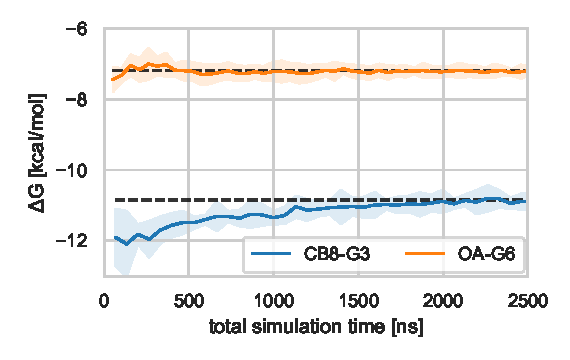
\includegraphics[width=0.95\linewidth]{fig6/free_energy_trajectories.pdf}
    \caption{Average binding free energy of 5 replicate Hamiltonian replica exchange calculations as a function of total simulation time (i.e. the sum of the simulation time of all replicas) for the two host-guest systems CB8-G3 and OA-G3. Shaded areas represent 95\% confidence intervals around the mean computed from the 5 replicates data. The horizontal dashed lines show the final binding free energy prediction of the two calculations after a total of ~5230 ns for OA-G3 and ~6650 ns for CB8-G3. Longer correlation times in CB8-G3 cause the calculation to converge more slowly. The original data used to generate the plot can be found at \url{https://github.com/MobleyLab/SAMPL6/blob/master/host_guest/Analysis/SAMPLing/Data/reference_free_energies.csv}.
}
    \label{fig:freeenergytrajectories}
\end{figure}

%%%%%%%%%%%%%%%%%%%%
%              Terminology                  %
%%%%%%%%%%%%%%%%%%%%
\section{Terminology and abbreviations}
\label{sec:tem-abbrev}
\begin{itemize}
\item Feature Box covering major technical terms and abbreviations
\item Examples:
\begin{itemize}
\item EXP, BAR, MBAR
\item Double decoupling, single-topology, dual-topology, hybrid-topology, coupled-topology
\item FEP (free energy peturbation), alchemical, AFE (alchemical free energy)
\end{itemize}
\end{itemize}
%%%%%%%%%%%%%%%%%%%%
%                Software                    %
%%%%%%%%%%%%%%%%%%%%
\section{Available software -- a summary}
\todo[inline]{Samar: write section}
\label{sec:software}
There are several softwares availble for carrying out alchemical free energy calculations. In this section we discuss some of the popular commercial and free tools along with their features. 
\begin{itemize}
\item Commercial:
   \begin{itemize}
    \item FEP+ is a tool offered by Schrodinger Inc. under a commercial license. It has an intuitive GUI which makes it easier for non-experts to run alchemical free energy calculations and analyze the results. It runs DESMOND MD package under the hood and hence parallelizes very well on the GPUs. 
    \end{itemize}
\item Free or low-cost for academics / commercial for industry:
	\begin{itemize}
	\item CHARMM has a variety of tools developed over the years. PERT module can be used to define initial and final states and define the intermediate lambda points. FREN and BAR modules can be used to analyze the data after the MD run. Lambda-dynamics based free energy calulation can be carried out using the BLOCK module.  
	\item TIES and AMBER FEW? (Peter Coveney)
	\item AMBER, including its new pmemd.cuda version support free energy calculation. 
	\end{itemize}
\item Free (libre) open source:
	\begin{itemize}
	\item PLUMED is an open source tool which enables the usage of a variety of MD engines. It is designed as a plugin for MD packages such that it analyzes the trajectory on the fly. It also offers a VMD based plugin for the computation of collective variables.   	
	\item SIRE
	\item YANK is a tool developed by John Chodera and group on the top of OpenMM MD package. It allows the users to write their inputs in easy-to-use YAML format. 
	\item CHARMM-GUI is a web based tool for setting up a variety of MD simulations. It can be used to generate CHARMM sctipts for solvation and ligand-binding free energy calculations. 
	\item GROMACS is a molecular simulation package with a significant number of free energy methods implemente. The LiveCOMS GROMACS tutorial has an example free energycalculation~\cite{LiveCOMS-gromacs}.
	\item pmx for mutations
	\end{itemize}
\item Setup tools
	\begin{itemize}
	\item FESetup: AMBER, gromacs, Sire
	\item Lomap/Lomap2 : Relative alchemical transformation graph planning
	\end{itemize}
\item Analysis tools:
	\begin{itemize}
	\item Free Energy Workflows: Sire-specific free energy map analysis using weighted path averages
	\url{https://github.com/michellab/freenrgworkflows}
	\item Alchemlyb: Multipackage free energy analysis
	\url{https://github.com/alchemistry/alchemlyb}
	\item pymbar: MBAR implementation, but have to roll your own analysis wrapper
	\url{https://github.com/choderalab/pymbar}
	\end{itemize}
\end{itemize}

\section{Online resources}
\begin{itemize}
\item \url{http://www.ks.uiuc.edu/Training/Workshop/Urbana_2010A/lectures/TCBG-2010.pdf}
\item Basic Ingredients of Free Energy Calculations: A Review (\url{DOI: 10.1002/jcc.21450})
\item Good Practices in Free-Energy Calculations (\url{DOI: 10.1021/jp102971x})
\item Alchemical Free Energy Methods for Drug Discovery: Progress and Challenges (\url{doi: 10.1016/j.sbi.2011.01.011})
\item Alchemistry wiki: \url{http://www.alchemistry.org/wiki/Best_Practices}
\end{itemize}

\section{Checklist}
\label{sec:checklist}
\todo[inline, color={green!20}]{ASJSM: @Volunteer This needs to be revised and expanded, some initial thoughts were just thrown in.}
An attempt at identifying most important checklist items.


% This provides a checklist which
% - spans a full page
% - consists of multiple sub-checklists
% - exists on a separate page
% This style of checklist will be especially helpful if you want to encourage readers to print and use your checklist in practice, as they
% can easily print it without also printing other material from your manuscript. However, other styles of checklist are also possible (below).
\begin{Checklists*}[p!]

\begin{checklist}{Step 0 -- Know what you want to simulate }
\textbf{What are the first questions that need addressing before setting up a molecular dynamics simulation}\\
Extensive explanation for the checklist questions can be found in Section~\ref{sec:step0}.
\begin{itemize}
\item Can I get the required accuracy with the simulation I want to carry out?
\item Have I properly prepared my protein and ligand systems?
\item Does my system contain any groups that require custom parameters?
\item What simulation protocol will provide the most evidence to answer my hypothesis?

\item And finally
\end{itemize}
\end{checklist}

\begin{checklist}{Simulation preparation}
\textbf{How do I get started setting up an alchemical free energy calculation}
Extensive explanation for the checklist questions can be found in Section~\ref{sec:step1}.
\begin{itemize}
\item Have I followed the Best practices for biomolecular simulation set up?
\item In a relative simulation, will I run into problems with clashing geometries in the ligand transformation or crystal waters?
\end{itemize}
\end{checklist}
\end{Checklists*}

\begin{Checklists*}[p!]
\begin{checklist}{Absolute simulations}
\textbf{What are the main things I need to consider for an absolute alchemical free energy calculation?}
Extensive explanation for the checklist questions can be found in Section~\ref{sec:step2}.
\begin{itemize}
\item Topology
\item Restraints
\item Standard state handling
\end{itemize}
\end{checklist}

\begin{checklist}{Relative simulations}
\textbf{What are the main things I need to consider for an relative alchemical free energy calculation?}
Extensive explanation for the checklist questions can be found in Section~\ref{sec:step2}.
\begin{itemize}
\item First thing
\item Also remember
\item And finally
\end{itemize}
\end{checklist}

\begin{checklist}{Analysis}
\textbf{This is all about analysis of the simulation}
Extensive explanation for the checklist questions can be found in Section~\ref{sec:step4}.
\begin{itemize}
\item Are my simulations converged enough?
\item Am I using the right analysis techniques?
\end{itemize}
\end{checklist}

\end{Checklists*}
\clearpage

\section*{Author Contributions}
%%%%%%%%%%%%%%%%
% This section mustt describe the actual contributions of
% author. Since this is an electronic-only journal, there is
% no length limit when you describe the authors' contributions,
% so we recommend describing what they actually did rather than
% simply categorizing them in a small number of
% predefined roles as might be done in other journals.
%
% See the policies ``Policies on Authorship'' section of https://livecoms.github.io
% for more information on deciding on authorship and author order.
%%%%%%%%%%%%%%%%

(Explain the contributions of the different authors here)

% We suggest you preserve this comment:
For a more detailed description of author contributions,
see the GitHub issue tracking and changelog at \githubrepository.

\section*{Other Contributions}
%%%%%%%%%%%%%%%
% You should include all people who have filed issues that were
% accepted into the paper, or that upon discussion altered what was in the paper.
% Multiple significant contributions might mean that the contributor
% should be moved to authorship at the discretion of the a
%
% See the policies ``Policies on Authorship'' section of https://livecoms.github.io for
% more information on deciding on authorship and author order.
%%%%%%%%%%%%%%%

(Explain the contributions of any non-author contributors here)
% We suggest you preserve this comment:
For a more detailed description of contributions from the community and others, see the GitHub issue tracking and changelog at \githubrepository.

\section*{Potentially Conflicting Interests}
%%%%%%%
%Declare any potentially competing interests, financial or otherwise
%%%%%%%

Declare any potentially conflicting interests here, whether or not they pose an actual conflict in your view.

\section*{Funding Information}
%%%%%%%
% Authors should acknowledge funding sources here. Reference specific grants.
%%%%%%%
FMS acknowledges the support of NSF grant CHE-1111111.

\bibliography{alchemical}

%%%%%%%%%%%%%%%%%%%%%%%%%%%%%%%%%%%%%%%%%%%%%%%%%%%%%%%%%%%%
%%% APPENDICES
%%%%%%%%%%%%%%%%%%%%%%%%%%%%%%%%%%%%%%%%%%%%%%%%%%%%%%%%%%%%

%\appendix


\end{document}
